\documentclass[12pt,upcase]{mitthesis}

\usepackage[utf8]{inputenc}
\usepackage{amsmath}
\usepackage{microtype}
\usepackage{graphicx}
\graphicspath{{./images/}}
\graphicspath{{./diagrams/}}
\graphicspath{{./irb-docs/}}
\graphicspath{{./code/}}
\usepackage{multirow}
\usepackage{rotating}
\usepackage{natbib}
\bibliographystyle{apa}
\usepackage{url}
\usepackage{booktabs}
\usepackage{tabularx}
\usepackage[]{pdfpages}

\usepackage{xcolor}
 \colorlet{punct}{red!60!black}
 \definecolor{background}{HTML}{EEEEEE}
 \definecolor{delim}{RGB}{20,105,176}
 \colorlet{numb}{magenta!60!black}

\usepackage{color}
 \definecolor{editorLightGray}{cmyk}{0.05, 0.05, 0.05, 0.1}
 \definecolor{editorGray}{cmyk}{0.6, 0.55, 0.55, 0.2}
 \definecolor{editorPurple}{cmyk}{0.5, 1, 0, 0}
 \definecolor{editorWhite}{cmyk}{0, 0, 0, 0}
 \definecolor{editorBlack}{cmyk}{1, 1, 1, 1}
 \definecolor{editorOrange}{cmyk}{0, 0.8, 1, 0}
 \definecolor{editorBlue}{cmyk}{1, 0.6, 0, 0}
 \definecolor{editorPink}{cmyk}{0, 1, 0, 0}

\usepackage{style}
%\usepackage{listings}
% JSON
% \lstdefinelanguage{json}{
%     basicstyle=\normalfont\ttfamily,
%     numbers=left,
%     numberstyle=\scriptsize,
%     stepnumber=1,
%     numbersep=8pt,
%     showstringspaces=false,
%     breaklines=true,
%     frame=lines,
%     backgroundcolor=\color{background},
%     literate=
%      *{0}{{{\color{numb}0}}}{1}
%       {1}{{{\color{numb}1}}}{1}
%       {2}{{{\color{numb}2}}}{1}
%       {3}{{{\color{numb}3}}}{1}
%       {4}{{{\color{numb}4}}}{1}
%       {5}{{{\color{numb}5}}}{1}
%       {6}{{{\color{numb}6}}}{1}
%       {7}{{{\color{numb}7}}}{1}
%       {8}{{{\color{numb}8}}}{1}
%       {9}{{{\color{numb}9}}}{1}
%       {:}{{{\color{punct}{:}}}}{1}
%       {,}{{{\color{punct}{,}}}}{1}
%       {\{}{{{\color{delim}{\{}}}}{1}
%       {\}}{{{\color{delim}{\}}}}}{1}
%       {[}{{{\color{delim}{[}}}}{1}
%       {]}{{{\color{delim}{]}}}}{1},
% }

% % JavaScript
% \lstdefinelanguage{JavaScript}{
%   morekeywords={typeof, new, true, false, catch, function, return, null, catch, switch, var, if, in, while, do, else, case, break},
%   morecomment=[s]{/*}{*/},
%   morecomment=[l]//,
%   morestring=[b]",
%   morestring=[b]'
% }

% \lstdefinelanguage{HTML5}{
%  language=html,
%  sensitive=true,   
%  alsoletter={<>=-+},   
%  morecomment=[s]{<!-}{-->},
%  tag=[s],
%  otherkeywords={
%   % General
%   % >,
%   % Standard tags
%    <!DOCTYPE,
%    </html, <html, <head, <title, </title, <style, </style, <link, </head, <meta, />,
%     % body
%     </body, <body,
%     % Divs
%     </div, <div, </div>, 
%     % Paragraphs
%     </p, <p, </p>,
%     % scripts
%     </script, <script,
%     % More tags...
%     <canvas, /canvas>, <svg, <rect, <animateTransform, </rect>, </svg>, <video, <source, <iframe, </iframe>, </video>, <image, </image>
%  },
%  ndkeywords={=,
%     % General
%     +=,
%     % HTML attributes
%     charset=, src=, id=, width=, height=, style=, type=, rel=, href=,
%     % SVG attributes
%     fill=, attributeName=, begin=, dur=, from=, to=, poster=, controls=, x=, y=, repeatCount=, xlink:href=,
%     % CSS properties
%     margin:, padding:, background-image:, border:, top:, left:, position:, width:, height:,
%     % CSS3 properties
%     transform:, -moz-transform:, -webkit-transform:,
%     animation:, -webkit-animation:,
%     transition:,  transition-duration:, transition-property:, transition-timing-function:,
%  },
% }

% \lstdefinestyle{thesiscode} {%
%  % General design
%  % backgroundcolor=\color{editorGray},
%  basicstyle={\footnotesize\ttfamily},   
%  frame=b,
%  % line-numbers
%  xleftmargin={0.75cm},
%  numbers=left,
%  stepnumber=1,
%  firstnumber=1,
%  numberfirstline=true,	
%  % Code design
%  identifierstyle=\color{black},
%  keywordstyle=\color{blue}\bfseries,
%  ndkeywordstyle=\color{editorGreen}\bfseries,
%  stringstyle=\color{editorOcher}\ttfamily,
%  commentstyle=\color{brown}\ttfamily,
%  % Code
%  language=HTML5,
%  alsolanguage=JavaScript,
%  alsolanguage=json,
%  alsodigit={.:;},	
%  tabsize=2,
%  showtabs=false,
%  showspaces=false,
%  showstringspaces=false,
%  extendedchars=true,
%  breaklines=true,
% }


% use fancyhdr, to enable page style stuff (below)
\usepackage{fancyhdr}
\setlength{\headheight}{15.2pt}
\renewcommand{\headrulewidth}{0pt}

\pagestyle{plain}

\begin{document}
% Sherman 1
% Revision 1.1  92/04/22  13:08:20  epeisach

% BE SURE TO READ THE UNIVERSITY'S RULES ON WHAT FIELDS ARE REQUIRED OR ENCOURANGED FOR YOUR DEPARTMENT

\title{Implementing a Web-Based\\ Model Slicer for \\ 3D Printers }

\author{Michael U.B. Meding}

\prevdegrees{B.S., University of Massachusetts Lowell (2015)}

\department{Department of Computer Science}

% If the thesis is for two degrees simultaneously, list them both
% separated by \and like this:
% \degree{Doctor of Philosophy \and Master of Science}
\degree{Master of Science}
\degreemonth{December}
\degreeyear{2016}
\thesisdate{December 1, 2010}

% If there is more than one supervisor, use the \supervisor command
% once for each.
\supervisor{Fred G. Martin}{Associate Professor}
\reader{ Jeff Brown}{Associate Professor} % reader is not necessary

% this is the department committee chairman, not the thesis committee chairman. 
\chairman{Jie Wang}{Department Chairman}

% Make the titlepage based on the above information.  If you need
% something special and can't use the standard form, you can specify
% the exact text of the titlepage yourself.  Put it in a titlepage
% environment and leave blank lines where you want vertical space.
% The spaces will be adjusted to fill the entire page.  The dotted
% lines for the signatures are made with the \signature command.
\maketitle

% The abstractpage environment sets up everything on the page except
% the text itself.  The title and other header material are put at the
% top of the page, and the supervisors are listed at the bottom.  A
% new page is begun both before and after.  Of course, an abstract may
% be more than one page itself.  If you need more control over the
% format of the page, you can use the abstract environment, which puts
% the word "Abstract" at the beginning and single spaces its text.

%% You can either \input (*not* \include) your abstract file, or you can put
%% the text of the abstract directly between the \begin{abstractpage} and
%% \end{abstractpage} commands.

% First copy: start a new page, and save the page number.
\newpage
\thispagestyle{empty}
\mbox{}
\newpage
\thispagestyle{empty}

% Second copy: start a new page, and reset the page number.  This way,
% the second copy of the abstract is not counted as separate pages.
\pagestyle{plain}
\newpage
\setcounter{page}{1}
\pagenumbering{roman}
\begin{abstractpage}
% meding 1
% $Log: abstract.tex,v $
% Revision 1.1  93/05/14  14:56:25  starflt
% Initial revision
% 
% Revision 1.1  90/05/04  10:41:01  lwvanels
% Initial revision
% 
%
%% The text of your abstract and nothing else (other than comments) goes here.
%% It will be single-spaced and the rest of the text that is supposed to go on
%% the abstract page will be generated by the abstractpage environment.  This
%% file should be \input (not \include 'd) from cover.tex.

3D printing currently has a large gap between software and hardware. A hobbyist machine can now be purchased for less than \$500 but having good software to drive it is hard to find. Currently the only competent and free slicing software available is Cura and Repetier Host. Currently, Cura has varied support on all platforms, and Repetier Host is intended only for Windows. Neither software have any web support nor will they be likely to have any support in the future as the slicing process requires a computer with a considerable amount of both graphical and computational power. The purpose of this research is to construct a web based slicing software and make it simple for users without any prior knowledge of 3D printing to take full advantage of their printer and as a result will make 3D printing much more approachable for users who are not computer savvy. Additionally, this opens up opportunities for educators in STEM programs to teach students about 3D printing in a simple and practical way.

\end{abstractpage}

%%%%%%%%%%%%%%%%%%%%%%%%%%%%%%%%%%%%%%%%%%%%%%%%%%%%%%%%%%%%%%%%%%%%%%
% -*-latex-*-




\chapter*{Acknowledgments}
\renewcommand{\thefootnote}{\fnsymbol{footnote}}

\paragraph{}
 The work in this thesis was only possible because of all the helpful and guiding members of the UMass Lowell Computer Science community. 
 Many people have helped me not just in research effort, but in introducing me to new thoughts and ideas that became foundational to this project. 

\paragraph{}
This research would not have been possible without the helpful guidance of Professor Fred Martin.
His passion for education has been a constant source of inspiration.
I would like to thank Jeff Brown for serving as my thesis reader.
I would especially like to thank Kelsea Gildawie for the late nights spent helping me put my thoughts on paper.
It would not have been possible to finish this research without her help.

\paragraph{}
I also wish to acknowledge my parents Uwe and Sally, who have always encouraged me to pursue my education.
  % -*- Mode:TeX -*-
%% This file simply contains the commands that actually generate the table of
%% contents and lists of figures and tables.  You can omit any or all of
%% these files by simply taking out the appropriate command.  For more
%% information on these files, see appendix C.3.3 of the LaTeX manual. 
\tableofcontents
\newpage
\listoffigures
\newpage
\listoftables

%\chapter*{Preface}
This research is an exploration in engineering education. My story leading to this research starts three years ago with a reading group on engineering and design where, as an undergraduate, I started learning about the current research in the field. Many of the foundational works of this study were first introduced to me in that reading group. I then spent two years working hands-on with middle school students and design activities. In an after-school program, I was a mentor for groups of 6th, 7th, and 8th graders, and provided them with experience in constructing and programming robots and robotic devices. This program covered many different concepts, from basic electricity to functional software design. Recently, I have been a part of a proposal writing process that exposed me to many different models of design, and showed me that there are significant and seemingly incompatible variations among many of them. From here my first concept for this research was conceived: to build a model of the design process as observed in middle-school students. %Keep original goal
This would be useful in the field of engineering education not just as another model, but as a tool to understanding this specific age of students. 	% Preface is not part of the standard. I invented it for myself. Use it if you want by uncommenting.

	% Redefine the "plain" pagestyle to have pagenum in the header, right
	\fancypagestyle{plain}{
		\fancyhf{}
		\fancyhead[R]{\thepage}
	}

	\setcounter{page}{1}
	\pagenumbering{arabic}
	\pagestyle{plain}
	
\chapter{Introduction}
\paragraph{}
Over the past few years, 3D printing, has become immensely popular due in part to its reduction in cost and its easy availability.
An enthusiast can now purchase a do it yourself (DIY) 3D printer kit for less than \$500 however, one major pitfall that remains is the software support which leaves much to be desired.
Most of the big name companies that used to hold all of the patents for 3D printers have retained the software patents but not the hardware patents. 
This creates a gap in knowledge between building the printer and running it.
This research has served as an exploration of what software existed in the open source for 3D slicing and using that software to build a web based 3D print slicer.
This will, effectively “democratize” the world of 3D printing, much in the same way that Google has democratized the way we search the web. 
In an article written by Harvard Business review, they theorize that this rise in the popularity of 3D printing will spur an industrial revolution as manufacturing becomes more personalized and decentralized \citep{daveni-2015}.

\paragraph{}
To print something on a 3D printer, there is a multi-step process that can be daunting to many first time users. 
The first step in the process is to either create or download a model.
Creating a model can be achieved with any standard 3D CAD software, such as AutoCAD or SolidWorks.
Downloading pre-existing models from an online repository can be done from websites such as Thingiverse or YouMagine.
Once a model file is obtained, it is time to “slice” the model.
Slicing is the act of taking this model file and splitting it up into many thin layers that the 3D printer can understand.
This process can only be executed by a dedicated slicing software which can often be complicated to use and difficult to install.
Once the file has been sliced, the resulting file is a G-code file, which is simply a set of movement instructions that the printer head must follow.
This file is then loaded to an SD card or sent via a print server similar to the way that a normal 2D printer is networked.
Once the G-code file has been loaded all, that is left is to hit print either manually using the printers interface for the SD card or by hitting print on the network interface for the file that was uploaded.

%Diagram of the basic 3D printing process to aid in the above explanation.
\begin{figure}[!ht]
  \centering
  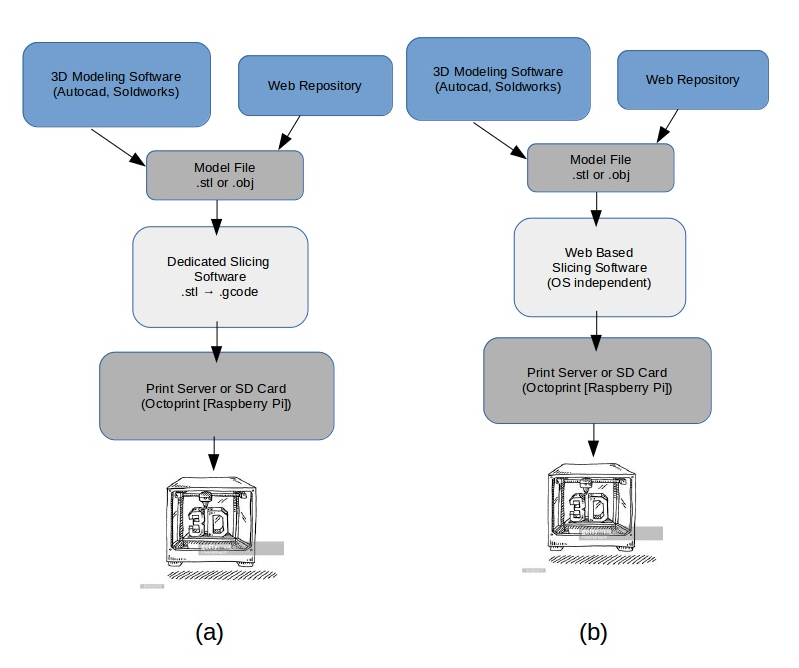
\includegraphics[width=\linewidth]{diagrams/basic-process-3D-printing}
  \caption{(a) High level view of the normal 3D printing process. (b) High level view of proposed new process using WebSlicer.}
\end{figure}


\section{The RepRap Idea}
\paragraph{}
The Replication Rapid-Prototyper Project (RepRap) is a movement with the goal of providing Open-source, diy 3D printers at low cost \citep{reprap-2011}.
RepRap printers are 3D printers with the additional ability to produce most of the parts necessary to assemble another identical printer.
This idea also extends outside of hardware but to the software as well.
Much of the software available for RepRap style printers are open source projects put together by the community.
Unfortunately, community based software development is slow and leads to hardware that outpaces its software.

\section{Sudden Growth of 3D Printing}
\paragraph{}
In an article written by Forbes, the market trend for 3D printing was analyzed.
They determined that 3D printing is becoming one of the fastest growing emerging markets, stating that
``The worldwide 3D printing industry is now expected to grow from \$3.07 billion in revenue in 2013 to \$12.8 billion by 2018, and exceed \$21 billion in worldwide revenue by 2020'' \citep{forbes3D}.
3D printing may be reaching more people as a result of the availability of the RepRap designs.
Additionally, building a 3D printer from a kit only requires basic hand tools and a moderate knowledge of electronics, which means that it has been opened up to a much broader audience.

\section{Purpose of Research}
\paragraph{}
The purpose of this research is to construct a web based slicer and simplify it for users who not well versed in 3D printing, so they are able to slice models and run their 3D printers.
This will make 3D printing much more approachable for occasional users who are not prepared to spend thousands of dollars on a professional machine and expensive software.
Additionally, this opens up opportunities for educators in STEM programs to teach students about 3D printing in a simple and practical way.
Under normal circumstances, this would not be a feasible project for a year-long Masters thesis; however, many of the technologies required to complete this project exist in varying states of completeness.
Combining them into a cohesive application will be the subject of this study.


\section{Research Objectives}
\paragraph{}
This research encountered several milestones which had to be met for it to be considered complete.
These milestones are listed in no particular order; however, several of them must be completed before allowing other milestones to be completed as detailed below.
However, several of them must be completed before allowing other milestones to be completed as detailed below.

\paragraph{}
CuraEngine is an open-source slicing engine designed to take model files in .stl file format and convert them into G-code for 3D printing.
For this project, wrapping this code and making it callable from the web is the heart of this application.

\subsection{Design Intuitive Web Interface}
\paragraph{}
This project requires both an intuitive and easy to way to slice a model file for 3D printing.
This would be completed using Bootstrap and AngularJS because they are both scalable and flexible for almost any web design.
These technologies also allow for small scale or even mobile use.

\subsection{Run Beta Testing with Actual Users}
\paragraph{}
No research would be complete without testing the software in question.
Running a closed beta test of this software is a milestone that must be met as one of the major aspects of this application is its usability.
The goals of this test were to see if WebSlicer is both easy to use and useful to those who decide to use it with their 3D printer.

\section{Related Work}
% Talk about Astroprint 2 and why its not the full solution.
\paragraph{}
%3.1 AstroPrint 2
%CITATION NEEDED
AstroPrint is an all-inclusive cloud operating system for 3D printers.
It attempts to encompass the entire package of 3D printing to a dedicated Raspberry Pi, or similar computer system.
It is also one of the only software platforms that currently exists that attempts to do web based slicing.
Unfortunately, the AstroPrint software tries to accomplish too many tasks at once and has become somewhat like a Swiss army knife, being capable of many functions but only complete a few tasks well.
Additionally, their cloud-based slicing software, while being reasonably fast, lacks any support for reviewing the sliced model.
This review stage is critical for anyone who is printing something that will take more than a few hours to complete.

\section{Thesis Map}
% This is where a design for reading this research should be shown so that someone can easily figure out what they want to read about.
% ideally this should be an ordered list similar to the index except more broad and with descriptions
\paragraph{}
\begin{itemize}
\item Chapter 2: Background and design choices.
	\paragraph{}
	This chapter discusses many of the external resources used and why they are relevant to this research.
\item Chapter 3: Software architecture review.
	\paragraph{}
	Compiled here is a complete overview of the architecture of WebSlicer. It follows the user through the entire process of slicing while explaining briefly some of the details of what is really happening.
\item Chapter 4: Client side in detail. 
	\paragraph{}
	Here is where all of the possible client interactions and application specific details are explained.
\item Chapter 5: Server side in detail.
	\paragraph{}
	Details of exactly how a C++ executable is tied into a Java process are explained here as well as the exposed web API created for this research.
\item Chapter 6: Discussion about usability testing and further improvements.
	\paragraph{}
	Included in this chapter are the formal results from closed beta testing and a discussion of the printer which inspired this research.
\end{itemize}


\chapter{Background}
\label{chap:background}

This chapter has been cut down significantly as this is just a template. You should write a LOT more than is here.

Education has evolved with culture and technology.  Classical wisdom calls only for the ``three R's" (reading, writing, and arithmetic) in schools, which today is considered foundational but insufficient for life. 

\section{Brief History of Engineering Education}

STEM education, of which engineering is a component, is in need of ``evidence-based" tools to measure their effectiveness \citep{csed-guzdial}. Conversely, lab-generated scientific data on education is often too abstract to be directly usable for real teachers \citep{sandoval}.

%\begin{figure}
%\centering
%\includegraphics[width=0.85\textwidth]{atman-senior-cycle}
%\caption{\label{fig:senior-cycle}Engineering process as observed in senior
%engineering students \citet{atman-2003}}
%\end{figure}

\section{Design Activity Studies}
	\label{sec:activity-design-studies}
\citet{welch} performed an experiment on design activities
carried out by seventh grade students. The steps are:

\begin{enumerate}
\item Understand the problem
\item Generate possible solutions
\item Model a possible solution
\item Build a solution
\item Evaluate the solution
\end{enumerate}

This paragraph shows how to use a label. A model-eliciting activity (MEA) is \label{sec:MEA}
designed such that the students' product is not a single
answer, but a rule or process that can be applied to solve similar
problems.

\section{This Study}
Many studies have examined the design process, providing a variety of insightful models and theories. 

\chapter{Methodology}
% This chapter is for going over my methods and talking about my software architecute and why it looks the way it does.

\section{Research Design} 
\paragraph{}
This thesis is a mixture of both research and design implementation.
The research portion of this project focused on linking an existing C++ application (CuraEngine) into a larger JavaEE based project.
This research also included running a closed beta test of the software and logging the results.

%Diagram of how the user interacts with WebSlicer from a high level .
\begin{figure}[!ht]
  \centering
  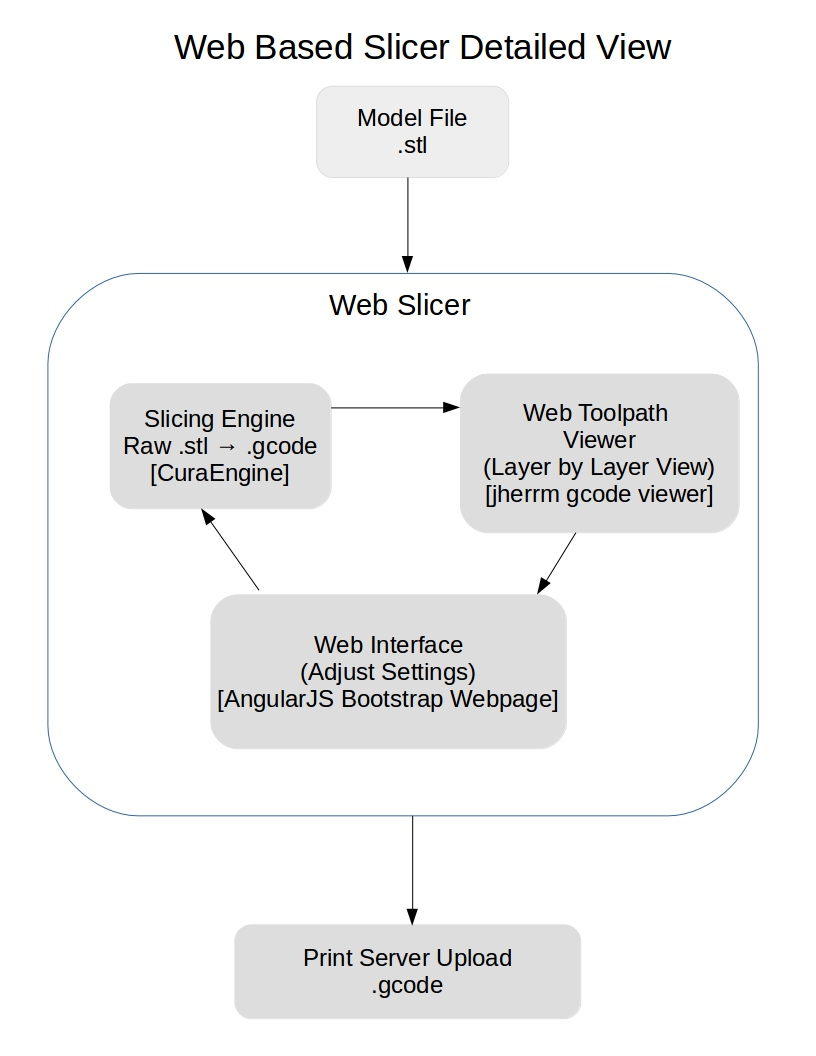
\includegraphics[width=\linewidth]{slicer-detailed-view}
  \caption{High level view of how WebSlicer functions and how users will interact with it}
  \label{fig:slicer-detailed-view}
\end{figure}

\section{Working procedure}
\paragraph{}
% this needs way more info
As shown in Figure \ref{fig:slicer-detailed-view}, the application will have 3 major components that all need to work together in a cycle until the user decides that the output is what they desire.

\subsection{Web Interface}
\paragraph{}
The web interface includes a set of forms for collecting the users settings for their printer and the settings as they relate to printing the model itself.
This interface also includes an interface so that the user may retain the files they have uploaded for future use.
This does not include the actual slicing engine which must be driven and accessed independently.

\subsection{Slicing Engine}
\paragraph{}
The slicing engine is at the heart of this project. 
It will include taking uploaded .stl model files by the user and convert them into raw G-code. 
The engine that carries out the raw geometry calculations is CuraEngine and is written in pure C++.
Thus, this portion of the project will required deploying CuraEngine on a remote server and creating a RESTful API to interface with it.

\subsection{Web Tool Path Viewer}
\paragraph{}
%expand this with more detail
After configuring and generating the G-code representation for a 3D model, there still must be a way to review visually how the slicing engine actually will split up the model.
This is done by loading the resulting gcode from the slicing engine into a web based visualizer.
The user is then able to view each of the layers and the steps involved in creating each one in detail.
From Figure \ref{fig:slicer-detailed-view} this process of changing settings, slicing, and reviewing can happen an arbitrary number of times before the user decides they are satisfied with the result.

\section{Review and Usability Testing}
\paragraph{}
After running through all steps of the working procedure it was then necessary to test WebSlicer by running a small beta test. 
This beta test consisted of a small group of users with varying familiarity with 3D printing to test how easy WebSlicer is to use through a series of simple tasks.
These simple tasks ranged from uploading a file to finding and adjusting the correct setting for a printer.

\chapter{Client Side}

\section{AngularJS, a bit of background}
\paragraph{}
To understand the structure of WebSlicer a few things must be known about how AngularJS applications are structured and a bit about how AngularJS itself works.
\cite{meding-2016} (2016), has more detailed explanations of each angular componenet than those that follow should the reader need more detail than that provided.

\subsection{Controllers \& Data Binding}
\paragraph{}
The controller structure in AngularJS sits in between the view and the JavaScript world acts like the glue between the two.
From a controller you are allowed access to "scope" variables which are like normal JavaScript variables but have a special two way data binding property.
Two way data binding is one of the most interesting features of AngularJS as it gives the user real time updates as the user interacts with a view.
In traditional JavaScript a developer has to listen for key events that occur in the browser as the trigger for a sequence of events.
Angular on the other hand also has a sequence of events but no trigger is required as the sequence of events is triggered automatically.
This action is known as a digest cycle.
The secret to this is that AngularJS has a watch for each variable attached to its scope and when any changes to this variable occur they propagate that change to the functions that are associated with that variable.

\subsection{Factories \& Services}
\paragraph{}
Plain JavaScript has many pitfalls but one of the most frustrating has to be the lack of any kind of larger design pattern support such as OOP (Object Oriented Programming).
The current trend with web based applications is to make single page applications with the same functionality as prior designs with many pages.
AngularJS is the answer to this with Factories and Services which mimic the design of a POJO (Plain Old Java Object) and Singleton objects in Java.

\subsection{Directives}
\paragraph{}
A directive is one of the most powerful structures in AngularJS.
It allows the programmer the power to write their own HTML5 tag with its own parameters and rules.
Directives also contain support for templates which are just short HTML snippets that replace the main tag when the code is loaded.
Combine this with the use of the aforementioned design patterns and it creates a very powerful tool to create and organize dynamic content.

\section{WebSlicer AngularJS Structure}
% this figure describes my full angular structure on the client
\begin{figure}[!ht]
  \centering
  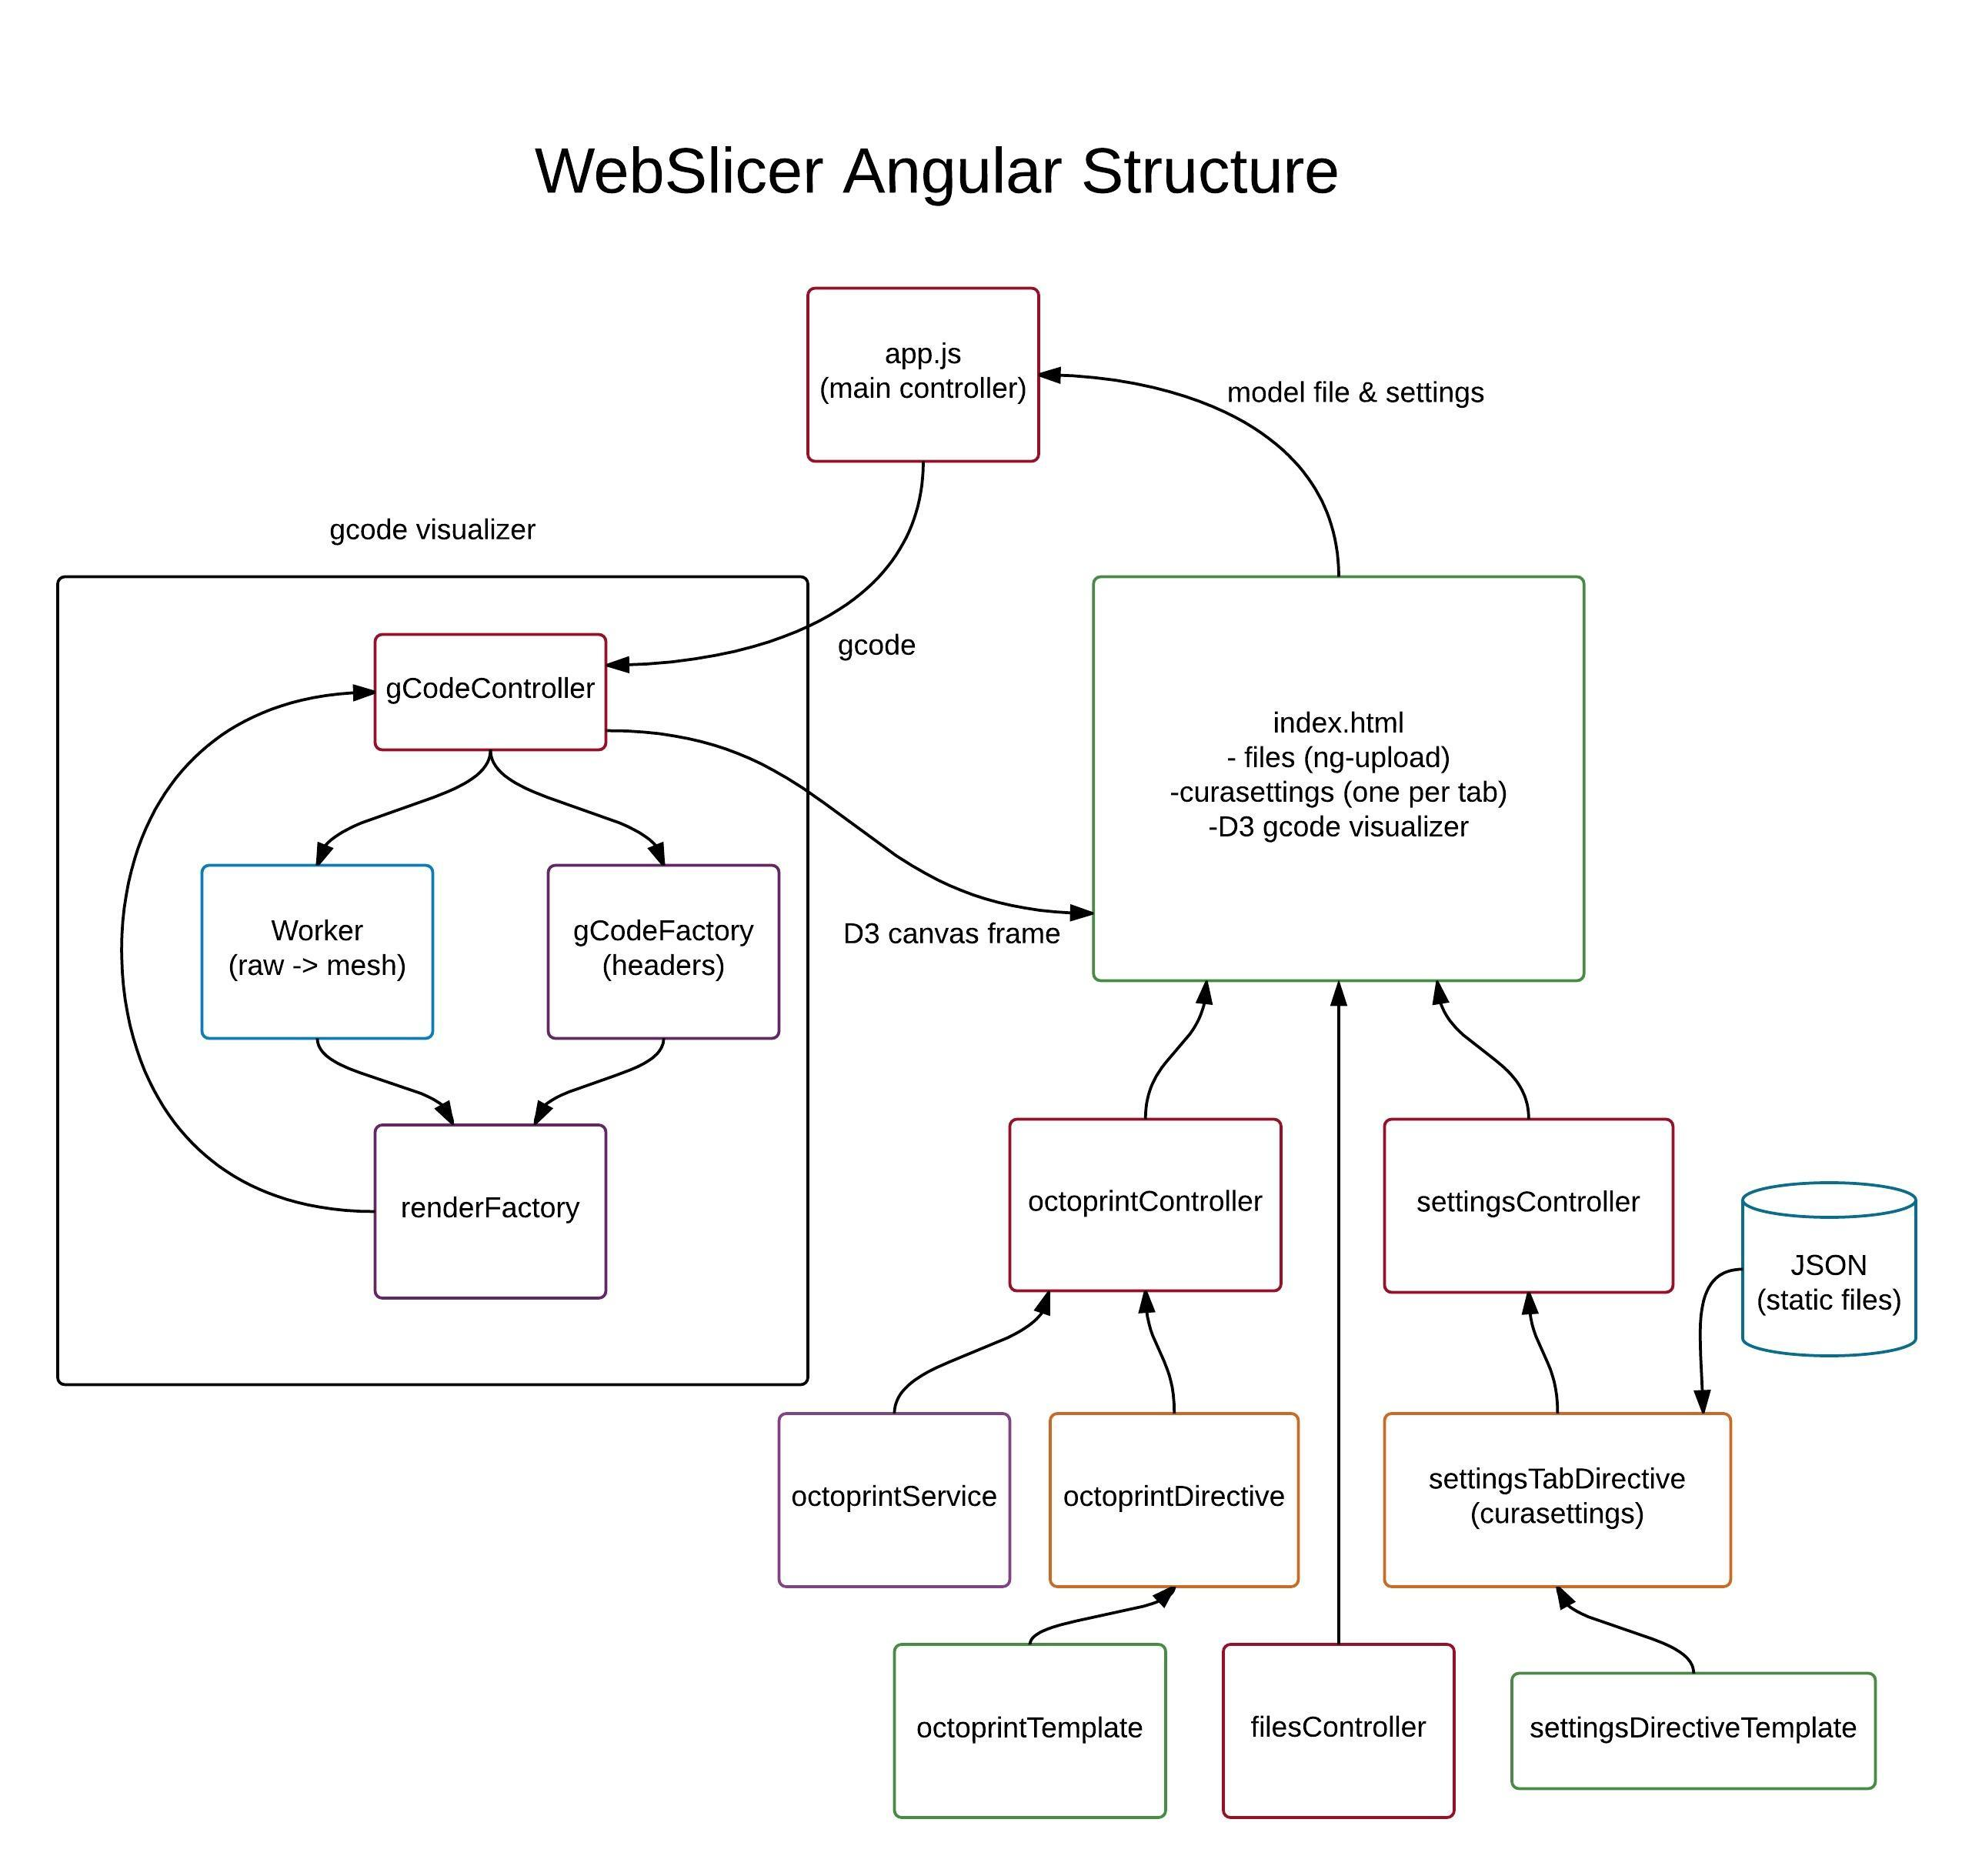
\includegraphics[width=\linewidth]{Client-Side-Structure}
  \caption{Full AngularJS structure breakdown}
  \label{fig:client-side-structure}
\end{figure}

\subsection{app.js}%app.js
The full graphical AngularJS structure of WebSlicer is shown in Figure \ref{fig:client-side-structure}.
Flow through this diagram starts with the app.js node which represents the main controller of the application.
This can be thought of as a main function in C++.
The main control variables are also inside of app.js which are similar to global variables.
Variables in this controller are used to store the current settings, file pointer, and output gcode.

\subsection{index.html}%index.html
Figure \ref{fig:client-side-structure} also shows that index.html is large hub and as WebSlicer is a single page web application this is the only static HTML file.
Index.html has several other functions such as bringing in all libraries and including the custom directives.

\subsection{Settings}%settings
% the flow of a settings throguh the application
\begin{figure}[!ht]
  \centering
  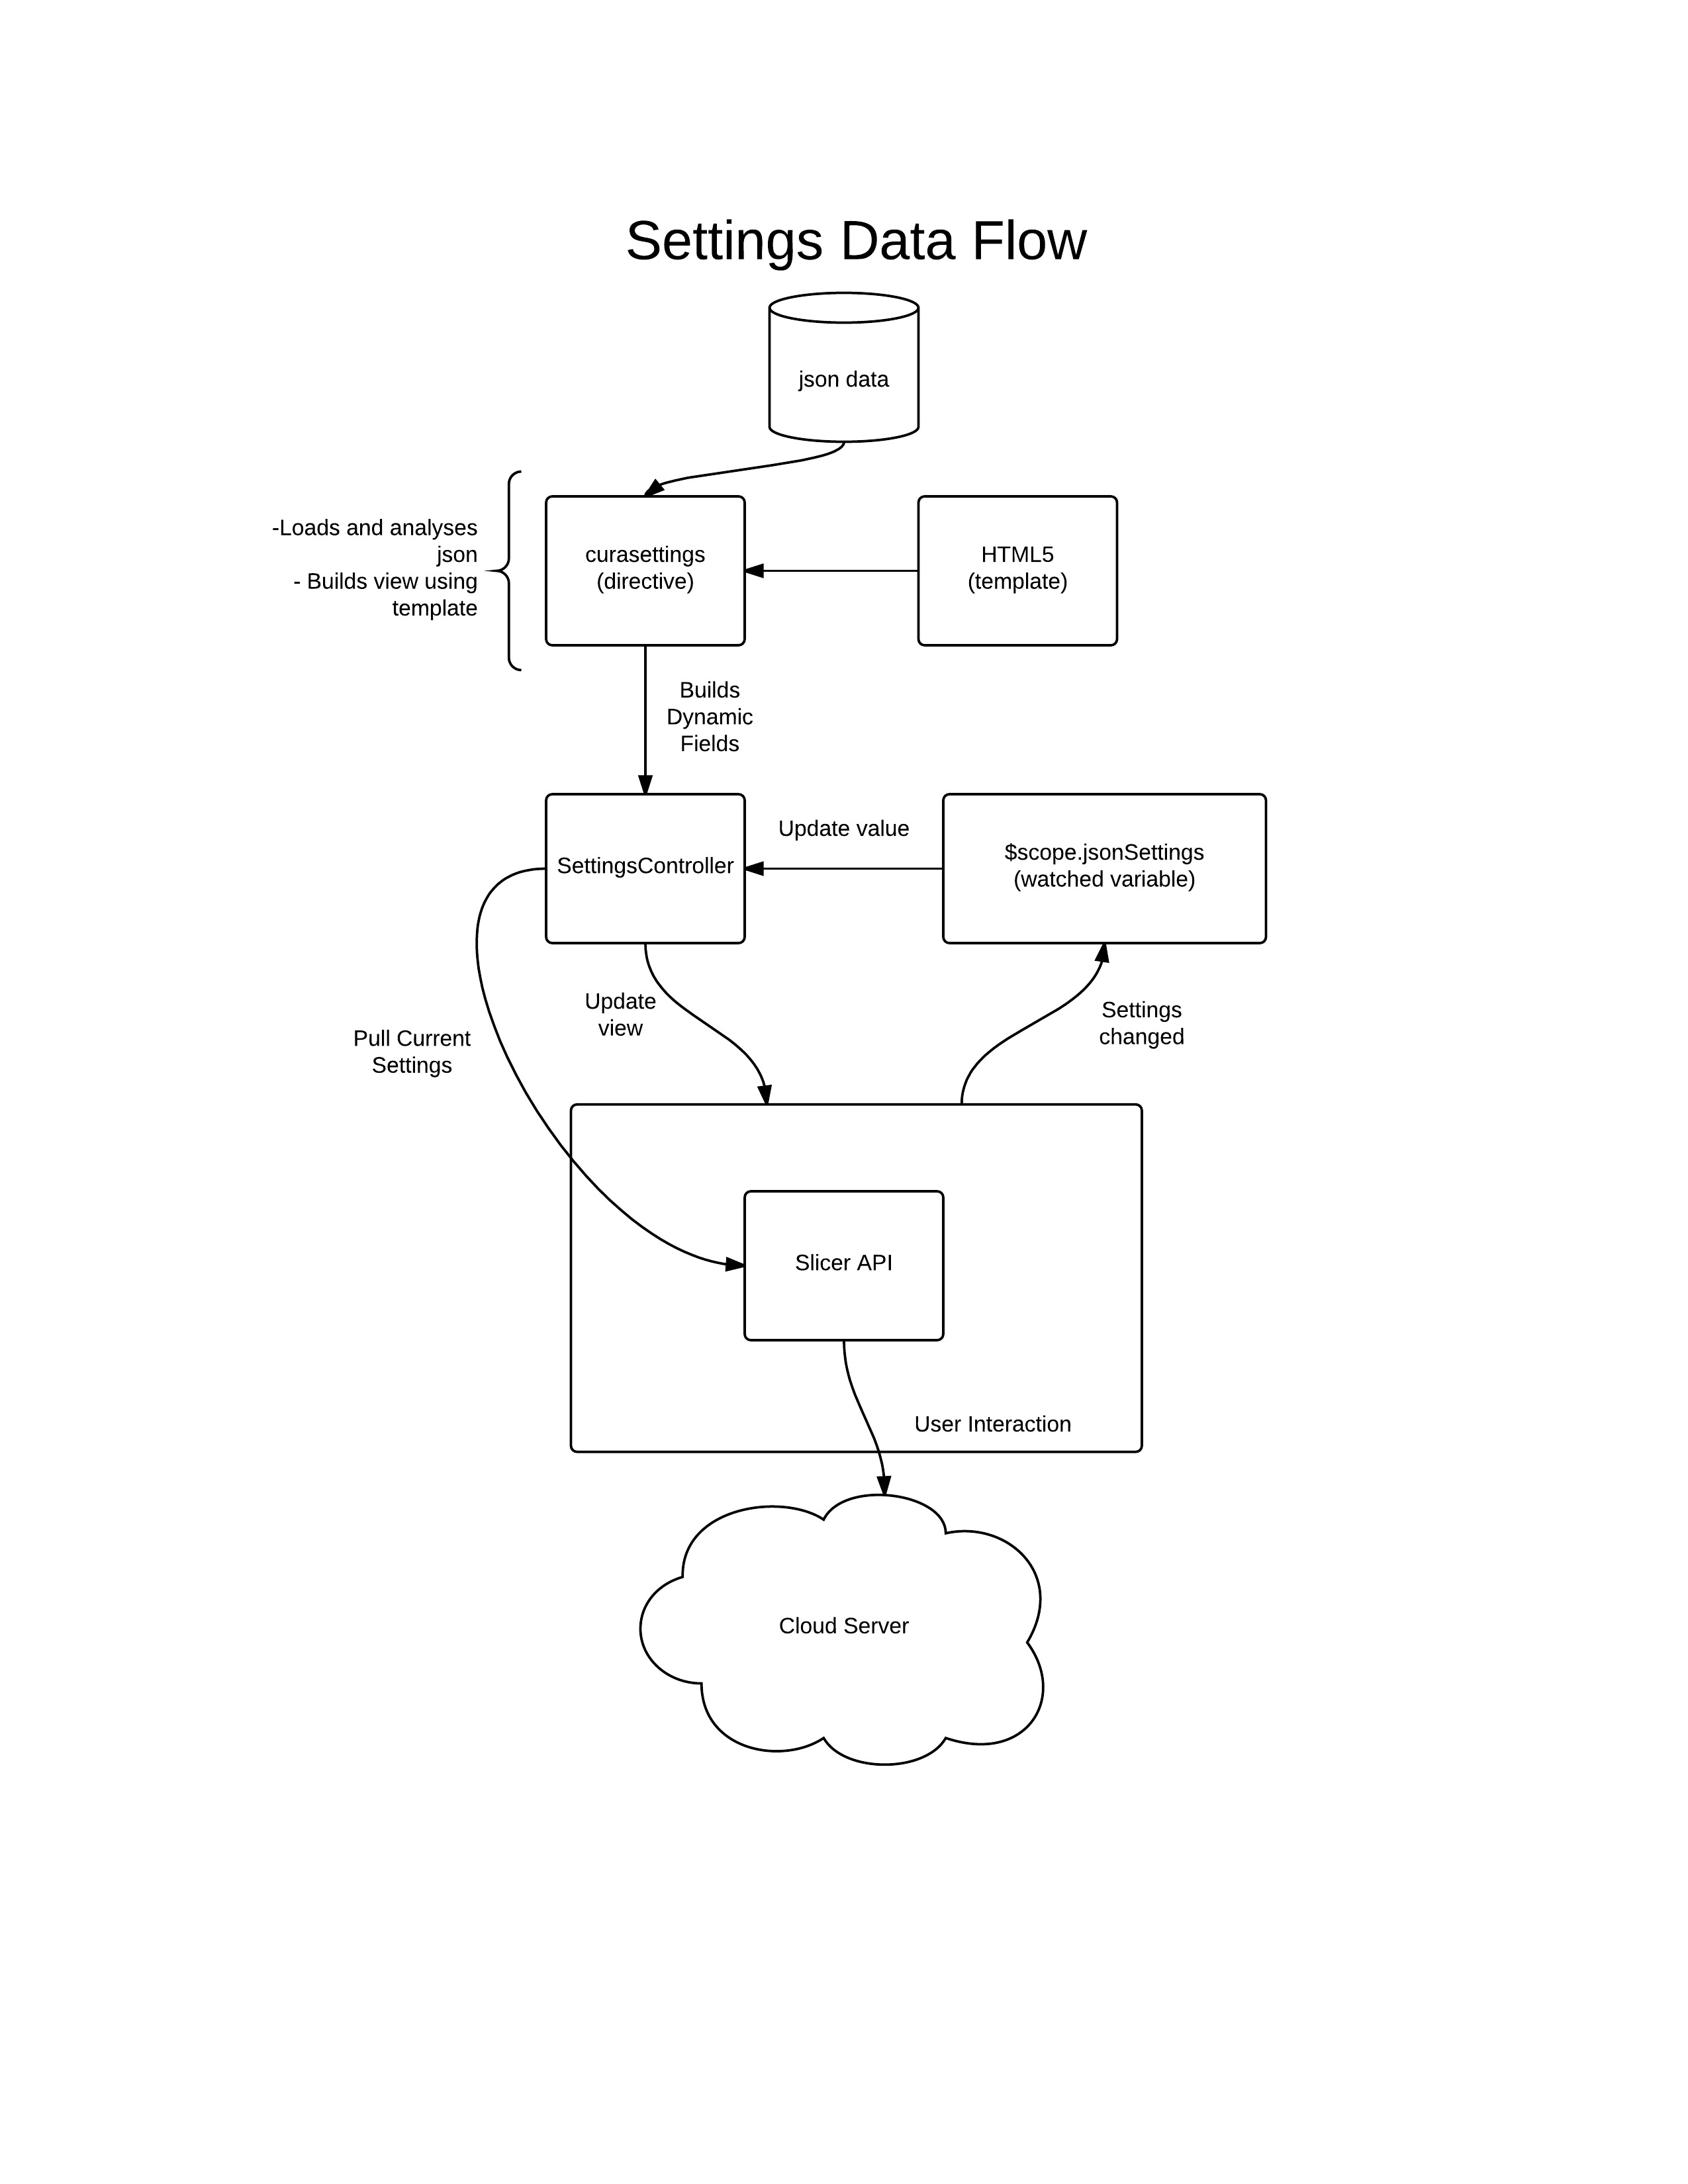
\includegraphics[width=\linewidth]{Settings-Data-Flow}
  \caption{The flow of data through the application from beginning to end of client side user interaction}
  \label{fig:settings-data-flow}
\end{figure}
\paragraph{}
As shown in Figure \ref{fig:settings-data-flow}, settings have a long path that they must travel behind the scenes before they are submitted to be used while slicing. 
This data flow starts with loading a static JSON (JavaScript Object Notation) file which describes the settings in a pattern as shown in Listing \ref{lst:json-settings}.
% JSON settings example listing
\begin{lstlisting}[language=json, style=thesiscode , label={lst:json-settings}, caption=A sample from a static settings file in JSON format.]
{
    "setting": "layer_height",
    "default": 0.1,
    "type": "float",
    "category": "Quality",
    "label": "Layer Height (mm)",
    "description": "Layer height in millimeters. This is the most important setting to determine the quality of your print. Normal quality prints are 0.1mm, high quality is 0.06mm. You can go up to 0.25mm."
}
\end{lstlisting}
% HTML example for how ng-repeat works
\begin{lstlisting}[language=HTML5, style=thesiscode, label={lst:html-repeat-example}, caption=An example of a ng-repeat looping construct in HTML5.]
<table class="table">
	<tr><td>Action</td><td>Done</td></tr>
	<tr ng-repeat="item in todos">
		<td>{{item.action}}</td>
		<td>{{item.done}}</td>
	</tr>
</table>
\end{lstlisting}

\paragraph{}
A directive called curasettings takes this static JSON file and splits it up so that for each setting object an input field exists in the template.
AngularJS provides this functionality through the use of an ng-repeat which is written in a similar fashion to that of a for loop in Python which is shown in Listing \ref{lst:html-repeat-example}.
Using a template for a directive in this case also meant that I could have control over many different kinds of fields such as drop downs and number specific inputs.
The curaengine directive also gave the logical separation of one static JSON file per tab of settings in the UI which made it simple to find and modify the settings as needed.

\paragraph{}
The interesting part about how settings work in WebSlicer is how they are tracked after being loaded to the client.
In most applications such as this there would be an individual watch on each field or a submit button which would trigger grabbing all the fields.
WebSlicer however uses a single object to track all of the settings for the application and uses a dynamic method of AngularJS to map from the input field to a field of a single object.
Thus when the settings are submitted there is no more interpolation needed as the settings object already has the current state as shown in the Figure \ref{fig:settings-data-flow} as "Pull Current Settings".

\subsection{Gcode Visualizer}
\paragraph{}
The gcode visualizer for WebSlicer is written using a combination of D3 and a JavaScript web worker.
From Figure \ref{fig:client-side-structure} it can be seen that the controller for the visualizer is sent a gcode file which it splits up to two separate services.
The controller itself does an initial parse of the file which places each one of the lines into its own entry in an array before passing it off to the gCodeFactory and Worker.
Both of these files parse through this entire array but do so at roughly the same time to speed along the process of visualizing.
The worker takes the array of lines and ignores the header to just focus on converting the raw movement commands into D3 lines so that they may be rendered.
The gCodeFactory takes the headers from the array and uses them to do analytics of the gcode file such as total print time.

\paragraph{}
The final steps in the process of visualizing the gcode require splitting the gcode file into layers for rendering.
A task which is made easy by simply following the meta tags in the gcode that signal a layer change and marking them in our array.
Once all of the heavyweight tasks of parsing and splitting up the gcode file are done it is simply a matter of returning layer requests with canvas frames.
Each time a layer is requested a progress for that layer is also sent.
The controller then just goes to the layer height in the array and renders a frame with the number of lines that are described by the current progress.
As array indexing is nearly instantaneous the visualizer once parsed and loaded runs very quickly to display layers.

\section{Key Challenges}
\subsection{Visualizer Integration}
\paragraph{}
By far one of the most difficult challenges overcome while writing WebSlicer was the visualizer integration.
The starter code for this was originally written by Nils Hitze as an open source project which had many other features \citet{hitzeViewer-2015}.
This code however required a lot of work to integrate properly with the rest of the application.
AngularJS despite its many features does not mingle well with other projects.
When all was said and done the only code which remained from the original was the JavaScript web worker and some of the parser code.

\subsection{Interpolating Settings}
\paragraph{}
Another difficult task when building this application was designing a method to handle a lot of input fields.
It would have been simple to just create a series of fields each with their own variable and submit methods and triggers but when settings change format and type it would have been an unmanageable mess very quickly.
So spending the extra time to design an intelligent method of handing large amounts of input data seemed logical.
This however ended up taking much more time and effort than anticipated.
At one point this even required getting in touch with the original developers of CuraEngine to ask them about what some of their settings meant.
Documentation for many of the settings was quite bad and in many instances was non existent which further slowed down development.

\section{Other Planned Integrations}
\subsection{OctoPrint}
\paragraph{}
A feature which was removed at a late state in the process of building this application was an integration with OctoPrint.
OctoPrint has a good API to allow for external applications to integrate easily with it making it an ideal choice for this application.
The idea of this integration was to allow a user who was running an OctoPrint server to be able to send files directly to their server.
This would eliminate the need of having to download the gcode from WebSlicer only to be uploaded to the print server seconds later.
It was decided at the last moment that this feature need not be in the minimum viable product and that time was best allocated to finishing more crucial features of the application.

\subsection{Thingiverse \& YouMagine}
\paragraph{}
Another planned integration was the ability to import from a web based repository such as Thingiverse or YouMagine.
These repositories are public sites where users can upload their 3D designs so that others can 3D print them.
Thingiverse in particular has a nice API for grabbing models from their site which would make it an easy integration for a web based slicing software.
However, this feature was given the axe early on as it would have required too much unnecessary development time to finish.

\section{Issues \& Known Bugs}
\paragraph{}
As mentioned in prior sections WebSlicer was designed with a minimum viable product in mind.
Developing a working 3D print slicer for the web was the primary task and all other features needed to support this or extend this functionality.
For this reason there is no login or user database which would normally be the first item to be developed for an application such as this.
There is also no way to view any of the models in 3D which for most users makes the software significantly harder to use.

\chapter{Server Side}
\begin{figure}[!ht]
  \centering
  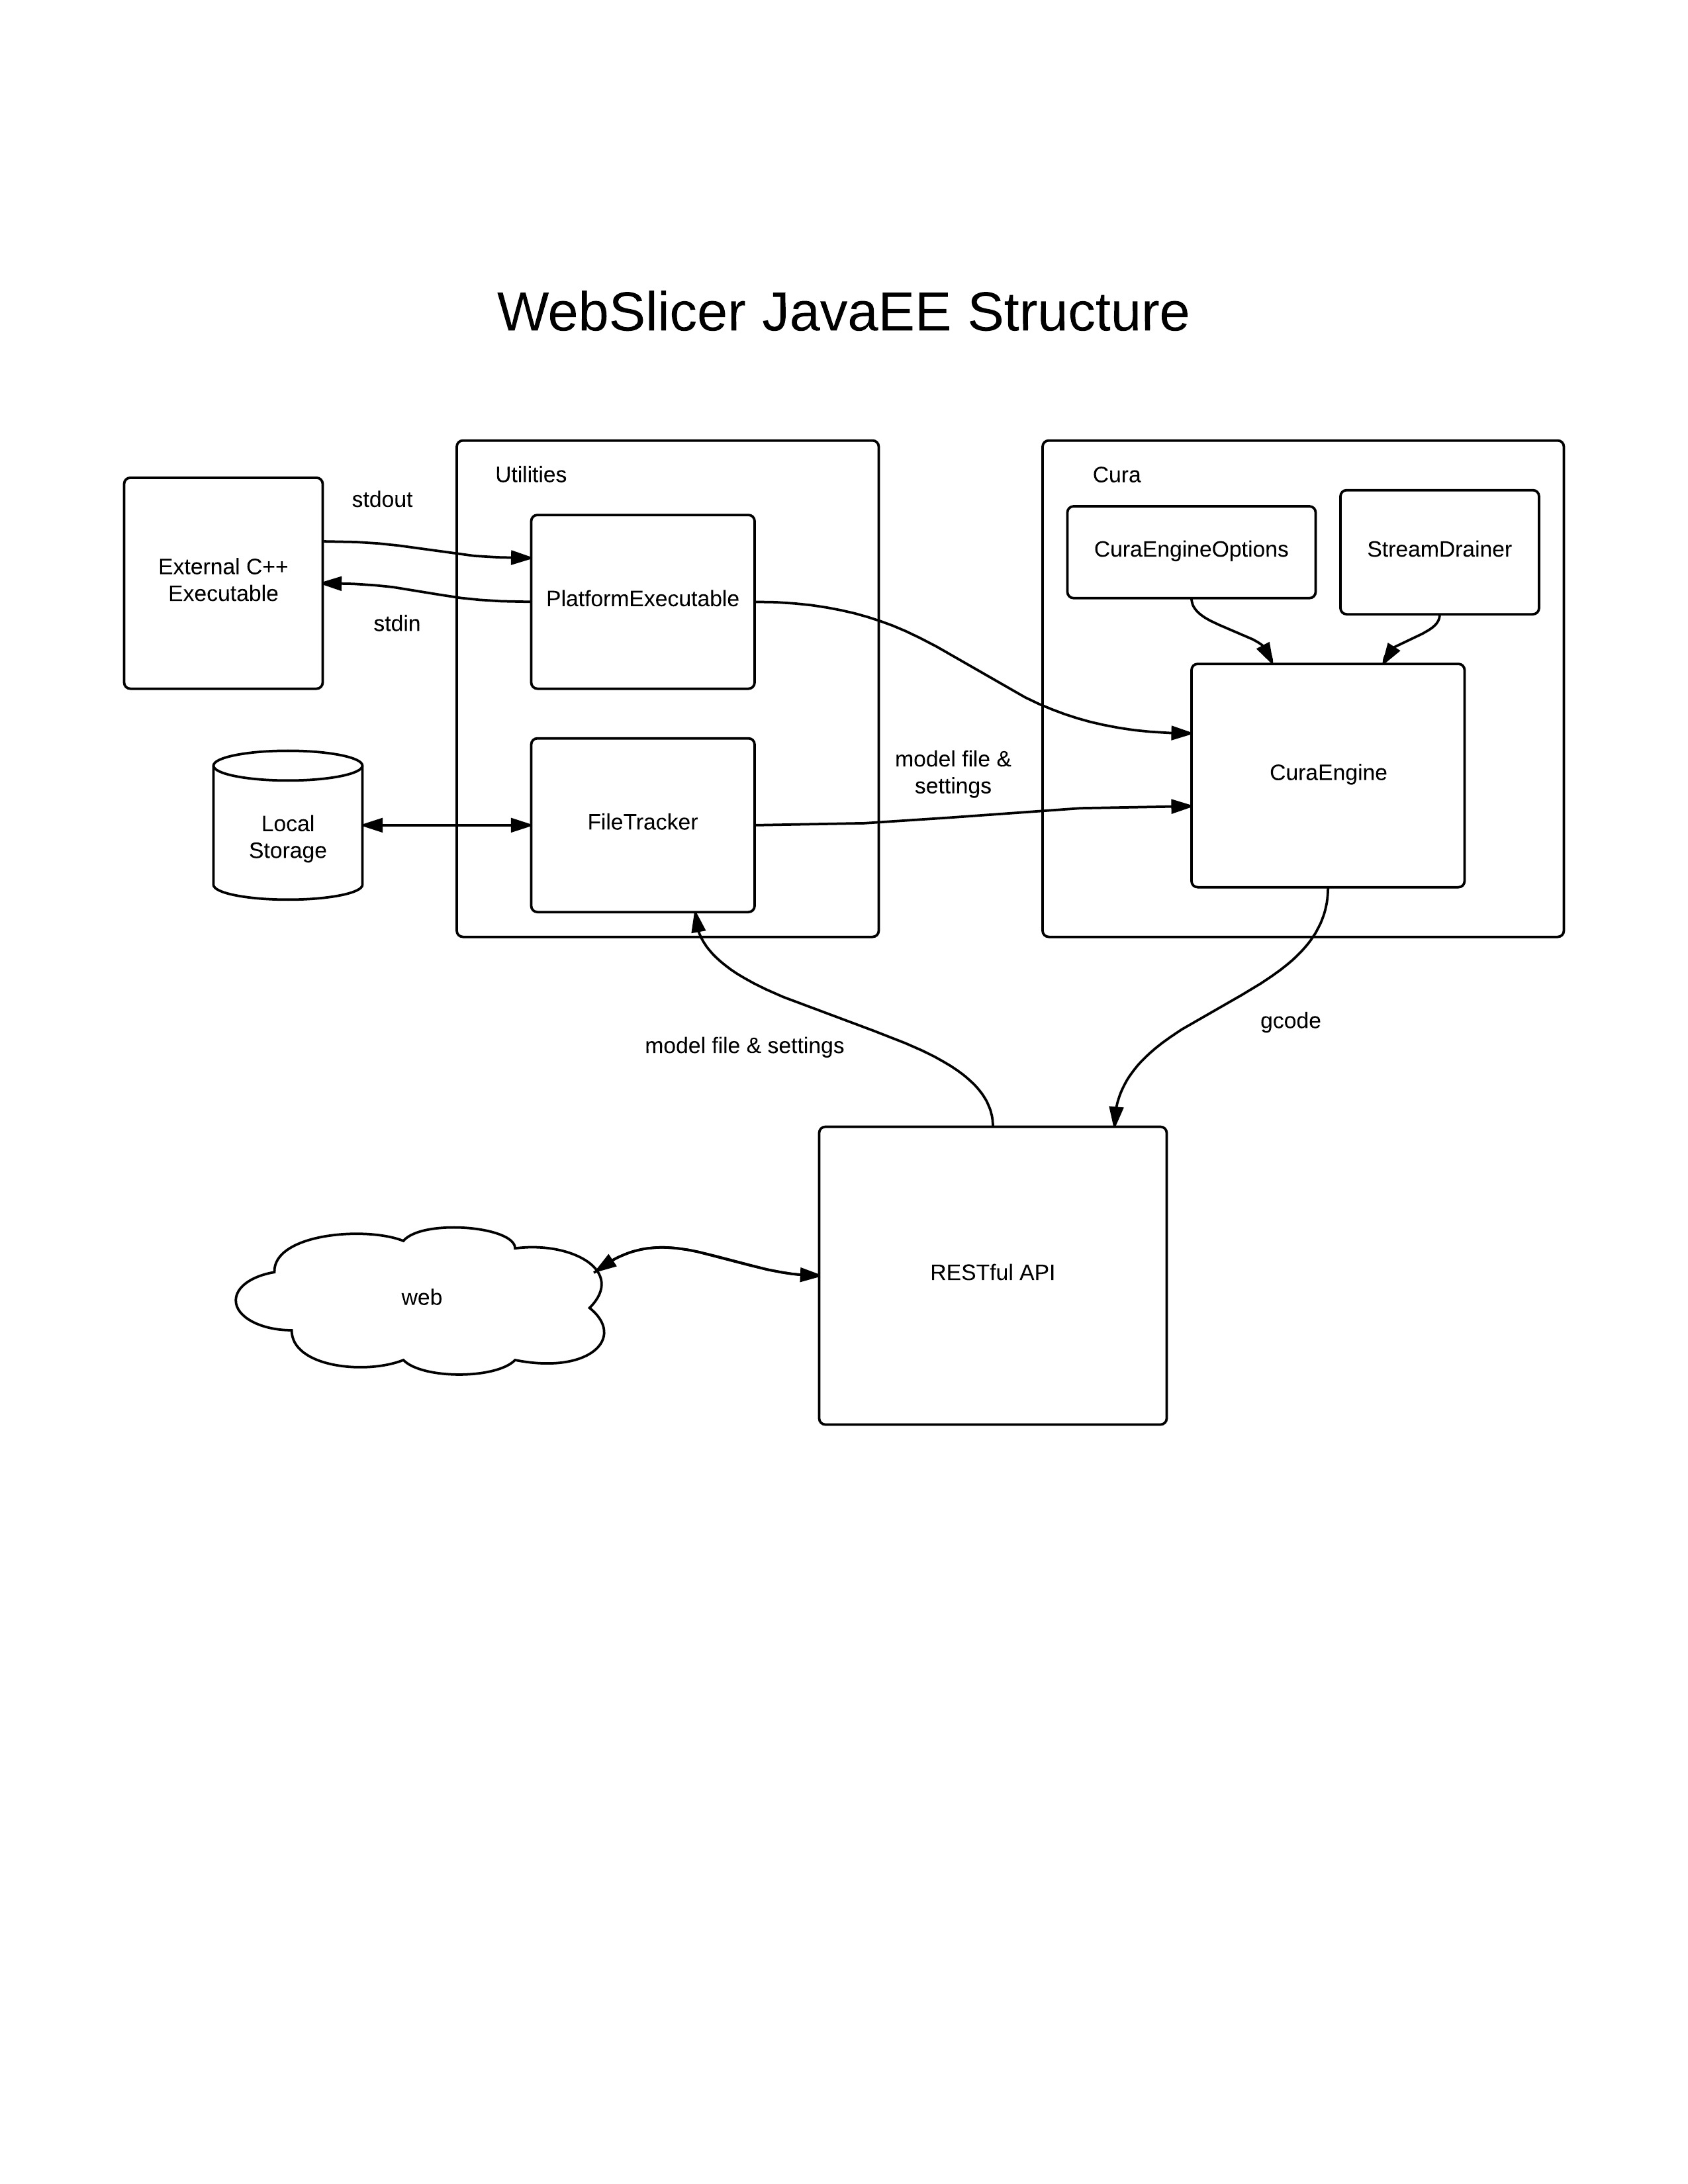
\includegraphics[width=\linewidth]{Server-Side-Structure}
  \caption{The structure of the server side of WebSlicer}
  \label{fig:server-side-structure}
\end{figure}

\section{JavaEE Structure}
\paragraph{}
The server side of WebSlicer was written in JavaEE, the structure for which is shown in Figure \ref{fig:server-side-structure}.
JavaEE was the optimal choice for this application as it allowed for the easiest deployment and was also the easiest to scale.
Additionally, JavaEE has a good code packaging mechanism for web and non web based applications alike.
The web container which is in use for this application exposes a RESTful API on a privately hosted server.

\paragraph{}
To further simplify the development process Maven was also used.
Maven is a build tool for Java and has support for deploying complex applications such as those in JavaEE.
This means that when a build was completed it was automatically deployed and ready for testing.

\section{ProcessBuilder}
\paragraph{}
At the core of the server side application is an executable called CuraEngine. 
It is the main executable which is compiled from the open source slicing platform Cura which is written in C++. 
This presented a problem as all of my server side code is written in Java. 
ProcessBuilder was the solution to this problem as it is capable of redirecting the input and output streams of a local executable process into my Java server application.
CuraEngine from Figure \ref{fig:server-side-structure} uses a ProcessBuilder and the PlatformExecutable to create a runnable Java method that is capable of executing like a C++ executable.
CuraOptions feeds the CuraEngine class with all of the parameters that it needs from the API.
It gathers the path to the appropriate settings file and includes all of the parameters needed to run the CuraEngine executable.
% running CuraEngine from the command line example
\begin{lstlisting}[language=bash, style=thesiscode, label={lst:curaengine-executable}, caption=An example of running CuraEngine C++ executable directly from the command line.]
CuraEngine slice -v -j {settings.json} -g -e -o {output.gcode} -l {model-file.stl}
\end{lstlisting}

\paragraph{}
An example of running the CuraEngine C++ executable from the command line is shown in Listing \ref{lst:curaengine-executable}.
When the ProcessBuilder class of WebSlicer recieves a slice command from the API it gathers the arguments listed in brackets and sends them to PlatformExecutable.
PlatformExecutable then spawns a native process and pipes its input and output streams into the respective Java streams.
At the same time StreamDrainer spawns a new thread and waits for the output stream that was created by PlatformExecutable.
StreamDrainer's task is to take the unneeded output from stdout and pipe it into a log file for debugging.

\paragraph{}
After CuraEngine has finished slicing the current file and PlatformExecutable has returned the REST API, which has been waiting, unblocks and starts reading the output gcode file.
This file is then packaged and sent back to the client as the response of the "/slice/\{clientId\}/\{modelId\}" command as shown in Table \ref{tab:restapi}.

\section{REST API}
% my REST API and the reason that I structured it the way I did
\begin{table}[h]
  \centering
    \begin{tabularx}{\textwidth}{ |l|l|X| }
      \hline
      Type & Address & Description \\ \hline
      \hline
      GET & /ping & A simple ping endpoint used for testing. \\ \hline
      POST & /setupClient & Sets aside all needed files for a new client and return its unique ID. \\ \hline
      POST & /importStl/\{clientId\} & Takes a MIME type file stream and imports the file to the clientId specificed in the URL. It also returns a unique identifier for the file. \\ \hline
      POST & /importSettings/\{clientId\} & Similar to importStl this endpoint takes a settings JSON file and imports it to the specificed clientId \\ \hline
      POST & /slice/\{clientId\}/\{modelId\} & This is the main slice function of the API. It combines all of the parameters specified by the calls before and returns a gcode file to the user. \\ \hline
      POST & /testSlice & A test endpoint that requires no parameters and simply returns some arbitary gcode to the user. \\ \hline
      GET & /getFiles/\{clientId\} & Returns all the model file names and their tracking ID's that are associated with a clientId. \\ \hline
    \end{tabularx}
  \caption{Documentation of all exposed endpoints of my RESTful API}
  \label{tab:restapi}
\end{table}

\paragraph{}


\section{Key Challenges}
\subsection{ProcessBuilder Deadlock}
\begin{figure}[!ht]
  \centering
  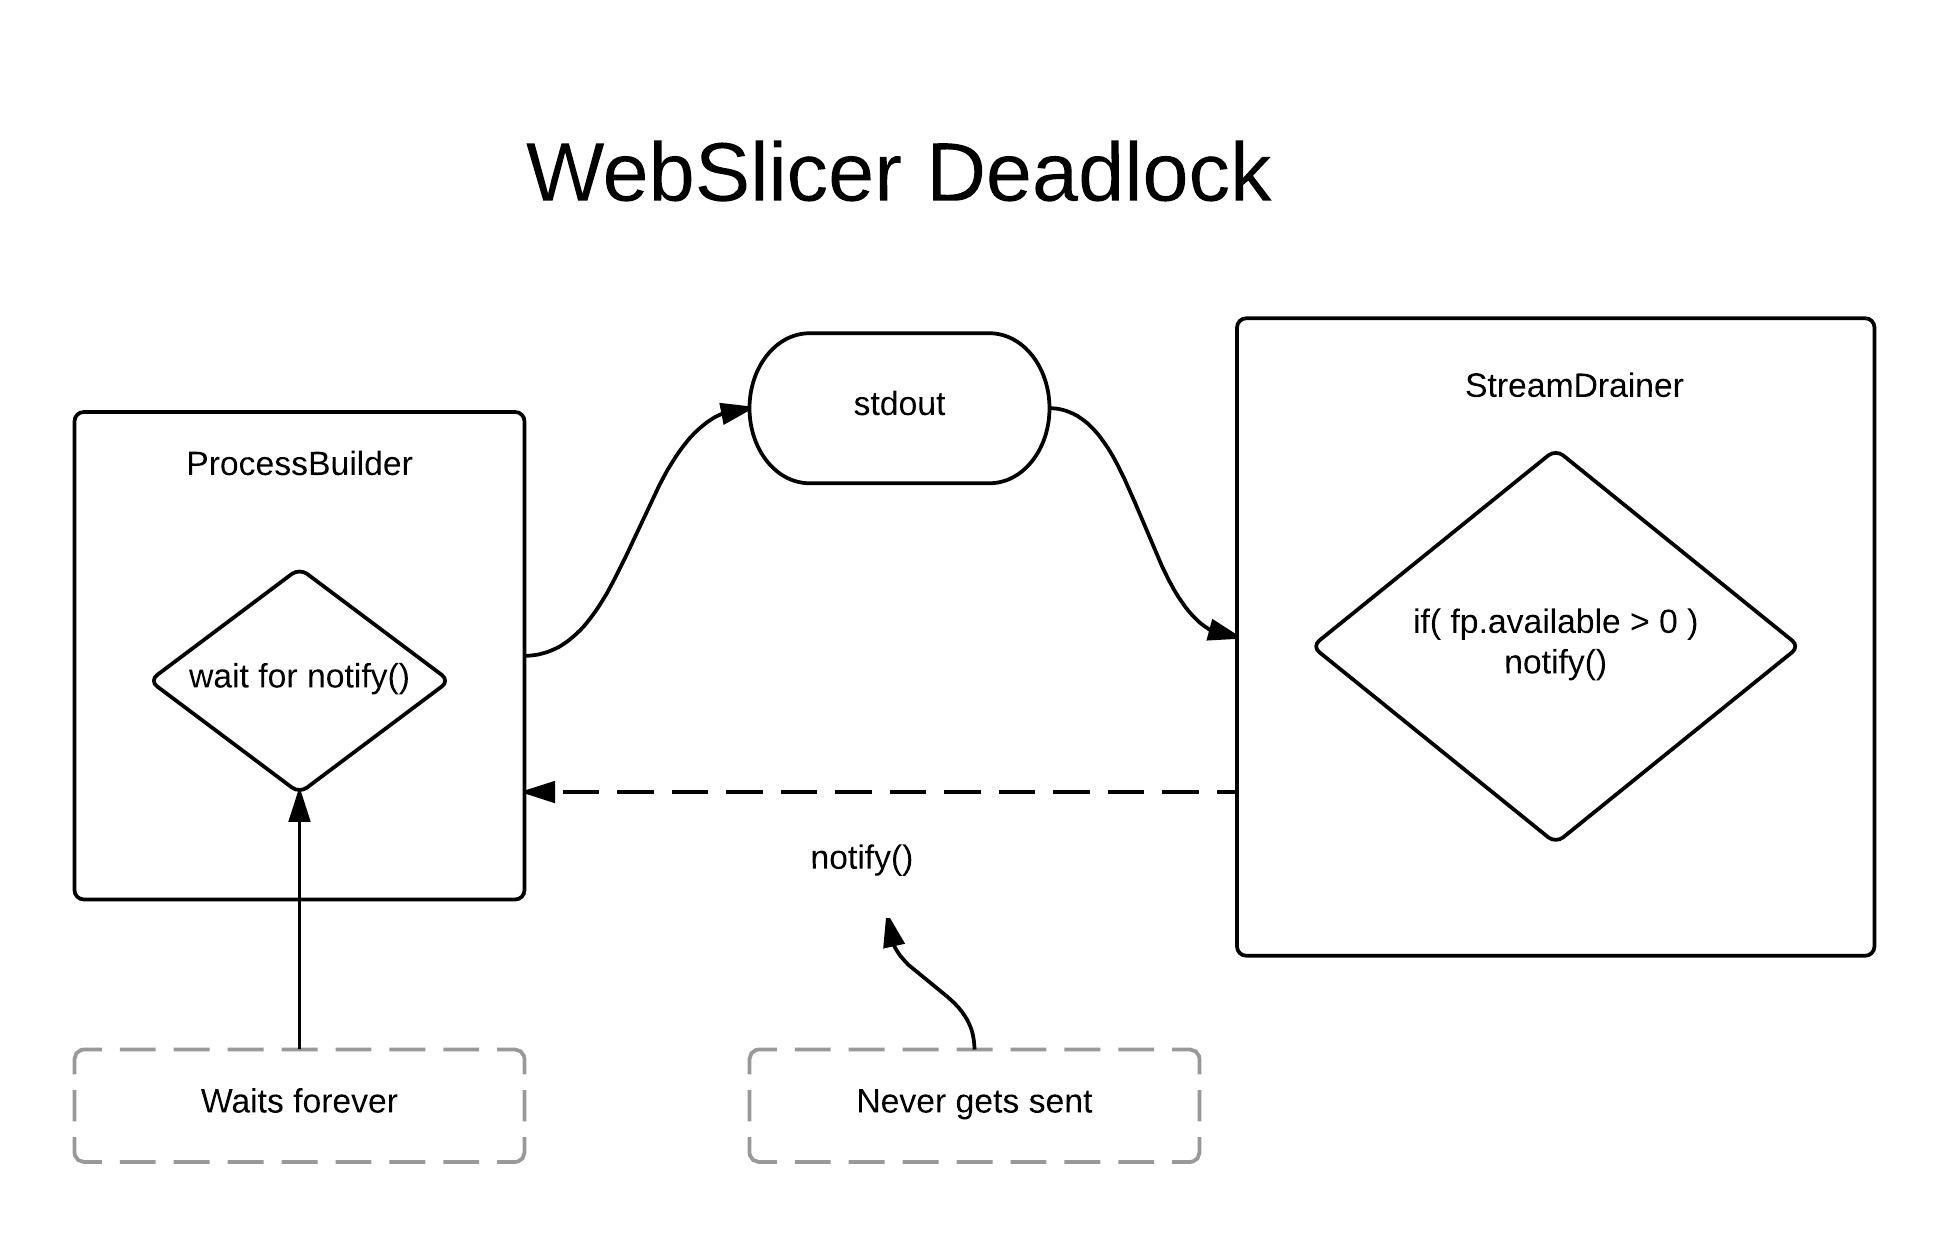
\includegraphics[width=\linewidth]{Deadlock-Diagram}
  \caption{Diagram of a deadlock issue that took weeks to resolve}
  \label{fig:deadlock-diagram}
\end{figure}
\paragraph{}
One of the biggest bugs encountered while developing this project was a thread deadlock issue. 
The server side code uses Javas ProcessBuilder which builds a system native call to an executable and then pipes the input and output into the input and output pipes of Javas stdio as shown in Figure \ref{fig:deadlock-diagram}.
This works very well for small platform executable’s with limited I/O but can become problematic when complex native calls such as the curaengine are used.

\paragraph{}
ProcessBuilder does its normal writes to stdout and the drainer just pipes them into a file. 
However the drainer has to wait for a file pointer using the fp.available() function. 
This is a non blocking function which only estimates the buffer size that it has for the file. 
The check for file pointer availablity was checking if this function returned something greater than 0 as an estimate before notifying the ProcessBuilder that it was ready. 
However the buffer size would often start as zero before allocation and as this check was not part of a loop it would stay stuck forever as the notify was missed.

\paragraph{}
This problem was solved by using the correct blocking file pointer available check. 
Occasionally the buffer size was larger than 0 and the application ran fine but with some models it would consistently fail as the buffer had not been allocated yet.
This solution is seemingly obvious yet this solution still took many days to find and correct as the application did not fail consistently.

\subsection{FileTracker Revamp}
\paragraph{}
The first iteration of FileTracker was a bit crude and not well planned out. 
It tracked two hashmaps, one for model files and the other for settings files with no mind for the client who actually needed to have access to those files. 
This worked fine for testing but had many pitfalls including the inablility to reuse files that already existed. 
As soon as the client died those files were lost which is a major inefficiency.

\paragraph{}
The fdmprinter.json file within the unique client folder is symbolically linked to the fdmprinter.json file within common. 
The CuraEngine executable requires that all of the settings files rest within the same directory when preforming a slice as shown in Listing \ref{lst:file-structure}.
This is somewhat problematic with the potential of having this file copied for many clients. 
Thus, symbolically linking the file to the rescue.

\paragraph{}
The output.gcode and settings.json files are dynamically overwritten for every iteration so their existence here is merely to please CuraEngine as it requires these files as arguments when preforming a slice. 
The user has no grasp of these files and is only able to access their content through the web interface which parses in and out of files.

% listing of the file structure that FileTracker creates
\begin{lstlisting}[language=html, style=thesiscode, label={lst:file-structure}, caption=WebSlicer's underlying file structure supported by FileTracker.]
webslicer/
- b1a2a69e-5893-4d7c-aa1f-d639fa3b4ed1/
  - fdmprinter.json -> /tmp/webslicer/common/fdmprinter.json
  - models/
     - balanced_die_version_2.stl
     - raldrich_planetary.stl
  - output.gcode
  - settings.json
- common/
  - fdmprinter.json
  - presets/
    - prusa_i3.json
    - ultimaker2.json
\end{lstlisting}

\section{Future Improvements}
\paragraph{}
Currently FileTracker does not take advantage of the presets within the common/presets/ folder as described by Listing \ref{lst:file-structure}. 
These files contain the default settings for the corresponding printer which right now are only the ultimaker2 and a basic configuration of a prusa i3 variant. 
Optimally, the user would select from one of these starting presets and then modify and save their own.
This would allow users an optimal starting point and lowering the amount of starting knowledge and increasing the usability of WebSlicer.

\paragraph{}
This new file structure also allowed for an easy client index. 
In the future the unique folder ID will become the client's identification number which will be tied to their login. 
Additionally, simplifying the login process with googles oauth 2.0 system was also planned.

\section{Issues \& Known Bugs}
\paragraph{}
Currently there is no way for the server to import existing user files into its structure.
This means that when the server is restarted for any reason that the entire supporting file structure with all user files is lost.
Resolving this is just a matter of writing an initial import function that indexes all of the existing files.
It was left out of the initial version due to time constraints.

\chapter{Discussion}

\section{Usability Testing}
\section{Data Gathering}
\section{Design Updates \& Improvements}
\section{Future Work}
% eventually this will become a small time manufacturing tool...



%% This defines the bibliography file (main.bib) and the bibliography style.
%% If you want to create a bibliography file by hand, change the contents of
%% this file to a `thebibliography' environment.  For more information 
%% see section 4.3 of the LaTeX manual.
\bibliographystyle{abbrvnat-quote}
%\bibliographystyle{plainnat}
\renewcommand{\bibname}{References}
\bibliography{bibliography}

\appendix
%\include{appendix-stub} 	%I used an appendix stub file before I wrote the real appendix so the main file would build correctly.
\chapter{IRB Compliance Documents}
\paragraph{}
Included with referances here are all the IRB compliance documents.

\section{Student Assent Form} \label{sec:student_assent}
	
	Figures \ref{fig:assent1} and \ref{fig:assent2} are the Student Assent Form completed by all of the participants in the study. 

        \includepdf[pages=-]{irb-docs/IRB-Exempt-Form.pdf}
	
%	\begin{figure}%  figure placement: here, top, bottom, or page
%   	\centering
%   		\fbox{
%   	\includegraphics[width=\textwidth]{IRB-Exempt-Form} 
%   		}
%   	\caption{Student assent form, page 1.}
%   	\label{fig:assent1}
%	\end{figure}
	
%	\begin{figure}%  figure placement: here, top, bottom, or page
%   	\centering
%   		\fbox{
%   	\includegraphics[width=\textwidth]{appendix/irb_student_assent2.pdf} 
%   		}
%   	\caption{Student assent form, page 2.}
%   	\label{fig:assent2}
%	\end{figure}

\chapter{Server Side Code Appendix}
\paragraph{}
Included in this appendix is the full source code written to run WebSlicer on a Wildfly application server.
The section names are the file locations as they exist from the top level directory.

% -----------------------------------------------------------------------------------------------------------------------------------------------------------
% CONFIG CODE
% -----------------------------------------------------------------------------------------------------------------------------------------------------------

\section{config/ApplicationConfig.java}
\lstsetjava
\begin{lstlisting}[language=Java, label={lst:ApplicationConfig}, caption=A required file in JavaEE for declaring the default application path when deployed.]
package com.partbuzz.slicer.config;


import javax.ws.rs.ApplicationPath;
import javax.ws.rs.core.Application;

/**
 * Created by mike on 1/9/16.
 */
@ApplicationPath("")
public class ApplicationConfig extends Application {
}
\end{lstlisting}


\section{config/CORSFilter}
\lstsetjava
\begin{lstlisting}[language=Java, label={lst:CORSFilter}, caption=As CuraEngine allows cross origin responses a filter is requred to allow access by default in WildFly.]
package com.partbuzz.slicer.config;

import java.io.IOException;

import javax.ws.rs.container.ContainerRequestContext;
import javax.ws.rs.container.ContainerResponseContext;
import javax.ws.rs.container.ContainerResponseFilter;
import javax.ws.rs.ext.Provider;

/**
 * @author mike
 */
@Provider
public class CORSFilter implements ContainerResponseFilter {

    @Override
    public void filter(final ContainerRequestContext requestContext,
                       final ContainerResponseContext cres) throws IOException {
        cres.getHeaders().add("Access-Control-Allow-Origin", "*");
        cres.getHeaders().add("Access-Control-Allow-Headers", "origin, content-type, accept, authorization");
        cres.getHeaders().add("Access-Control-Allow-Credentials", "true");
        cres.getHeaders().add("Access-Control-Allow-Methods", "GET, POST, PUT, DELETE, OPTIONS, HEAD");
        cres.getHeaders().add("Access-Control-Max-Age", "1209600");
    }

}
\end{lstlisting}

% -----------------------------------------------------------------------------------------------------------------------------------------------------------
% CURA CODE
% -----------------------------------------------------------------------------------------------------------------------------------------------------------

\section{cura/CuraEngine.java}
\lstsetjava
\begin{lstlisting}[language=Java, label={lst:CuraEngine}, caption=CuraEngine.java is the main code that preforms slicing throgh the CuraEngine C++ executable.]
/*
 * Copyright (c) 2016 Michael Meding -- All Rights Reserved.
 */
package com.partbuzz.slicer.cura;

import com.partbuzz.slicer.util.CuraEngineException;
import com.partbuzz.slicer.util.PlatformExecutable;

import java.io.IOException;
import java.io.InputStream;
import java.util.ArrayList;
import java.util.List;
import java.util.logging.Logger;

/**
 * Invoke the CURA slicing engine.
 * <p>
 * SAMPLE BASH
 * ../../CuraEngine-master/build/CuraEngine slice -v -j ultimaker2.json -g -e -o "output/test.gcode" -l ../../models/ControlPanel.stl
 *
 * @author mike
 */
public class CuraEngine extends PlatformExecutable {

    private static final Logger log = Logger.getLogger(CuraEngine.class.getName());
    private static final String CURAENGINE_PROG = "/usr/local/bin/CuraEngine";
    private final CuraEngineOptions options;

    public CuraEngine() {
        this.options = new CuraEngineOptions();
    }

    public CuraEngineOptions options() {
        return options;
    }

    public String output = "";

    /**
     * Setup a stream drainer.
     *
     * @param fp the input stream
     * @return the stream drainer
     * @throws java.io.IOException
     */
    protected static StreamDrainer setupStreamDrain(InputStream fp) throws IOException {
        final StreamDrainer drainer = new StreamDrainer(fp);
        // wait until we are draining
        synchronized (drainer) {

            log.info("starting thread");
            Thread t = new Thread(drainer);
            t.setDaemon(true);
            t.start();

            while (!drainer.hasStarted()) {
                try {
                    log.info("waiting for drainer thread");
                    drainer.wait(500);
                    log.info("drainer wait expired");
                } catch (InterruptedException ex) {
                    Thread.interrupted();
                    throw new IOException("Unable to setup stream drainer");
                }
            }

            log.info("drainer started");
        }

        return drainer;
    }

    /**
     * Run the CURA engine.
     *
     * @throws CuraEngineException
     */
    public void execute() throws IOException {
        checkPlatformExecutable(CURAENGINE_PROG);

        List<String> arguments = new ArrayList<>();
        arguments.add(CURAENGINE_PROG); // add base executable
        arguments.addAll(options.getOptions()); // add all options in the correct order

        for (String arg : arguments) {
            log.info("cura argument: " + arg);
        }

        // Process builder options for command line execution
        ProcessBuilder pb = new ProcessBuilder();
//		pb.directory(basePath);
        pb.redirectErrorStream(true);
        pb.command(arguments);

        // Create new thread and start execution
        Process p = pb.start();
        try {

            // Setup drains for both output and error streams
            StreamDrainer stdout = setupStreamDrain(p.getInputStream());
//            StreamDrainer stderr = setupStreamDrain(p.getErrorStream());

            int status = p.waitFor(); // wait for slice to finish

            if (status == 0) {

                // gather everything that is sent back from the command.
                StringBuilder sb = new StringBuilder();
                InputStream fp = p.getInputStream();
                byte[] buffer = new byte[512];
                while (fp.available() > 0) {
                    int n = fp.read(buffer);
                    sb.append(new String(buffer, 0, n));
                }
                output = sb.toString();
                log.info(output); // just log the output for now
                log.info("STDOUT:" + stdout.getText());
                return;
            } else {
                throw new CuraEngineException("unable to parse gcode file");
            }

//            if (options.haveIgnoreErrors()) {
//                log.warning(sb.toString());
//            } else {
//                throw new CuraEngineException(sb.toString());
//            }


        } catch (InterruptedException e) {
            throw new IOException(e);
        } finally {
            cleanupResources(p);
        }
    }

    /**
     * After execute is called the standard out of the call is concatenated into output.
     *
     * @return
     */
    public String getOutput() {
        return output;
    }
}
\end{lstlisting}


\section{cura/CuraEngineOptions.java}
\lstsetjava
\begin{lstlisting}[language=Java, label={lst:CuraEngineOptions}, caption=All arguments to the CuraEngine C++ executeable must be compiled before it can be executed. This code is the compiler for that argument list.]
package com.partbuzz.slicer.cura;

import com.partbuzz.slicer.util.CuraEngineException;

import java.util.ArrayList;
import java.util.List;

/**
 * Created by mike on 3/30/16.
 */

public class CuraEngineOptions {

    private String settingsFileName;
    private String outputFileName;
    private String modelFileName;
    private boolean verbose = false;
    private boolean p_option = false;
    private boolean g_option = false;
    private boolean e_option = false;
    private boolean ignoreErrors = false;

    /**
     * Set the verbose mode.
     *
     * @return the options
     */
    public CuraEngineOptions verbose() {
        this.verbose = true;
        return this;
    }

    /**
     * Set the settings file. This is a JSON formatted file which includes all needed information for slicing the file.
     *
     * @param filename the settings filename
     * @return the options
     */
    public CuraEngineOptions settingsFilename(String filename) {
        this.settingsFileName = filename;
        return this;
    }

    /**
     * Set the output filename. The resulting gcode file name/location.
     *
     * @param filename the output filename
     * @return the options
     */
    public CuraEngineOptions outputFilename(String filename) {
        this.outputFileName = filename;
        return this;
    }

    /**
     * Set the model filename. This is the model to be sliced.
     *
     * @param filename
     * @return options
     */
    public CuraEngineOptions modelFilename(String filename) {
        this.modelFileName = filename;
        return this;
    }

    /**
     * This option is similar to verbose but instead of just logging the output to the screen it logs the output to the CuraEngine log files.
     *
     * @return the options
     */
    public CuraEngineOptions logProgress() {
        this.p_option = true;
        return this;
    }

    /**
     * Switch setting focus to the current mesh group only.
     * Used for one-at-a-time printing.
     *
     * @return the options
     */
    public CuraEngineOptions currentGroupOnly() {
        g_option = true;
        return this;
    }

    /**
     * Adds a new extruder train for multi extrusion. For every time -e is included another extruder is added as on option to the slicer.
     *
     * @return the options
     */
    public CuraEngineOptions extruderTrainOption() {
        e_option = true;
        return this;
    }

    /**
     * For debugging.
     *
     * @return the options
     */
    public CuraEngineOptions ignoreErrors() {
        this.ignoreErrors = true;
        return this;
    }

    public boolean haveIgnoreErrors() {
        return ignoreErrors;
    }

    /*
     * Get the options in the right sequence. To build a correct CuraEngine command line executable.
     */
    public List<String> getOptions() throws CuraEngineException {
        List<String> list = new ArrayList<>();
        list.add("slice"); // the main parameter of the CuraEngine executable.
        if (verbose) {
            list.add("-v");
        }
        if (p_option) {
            list.add("-p");
        }

        if (settingsFileName == null) {
            throw new CuraEngineException("no setting file defined");
        } else {
            list.add("-j");
            list.add(settingsFileName);
        }
        if (g_option) {
            list.add("-g");
        }
        if (e_option) {
            list.add("-e");
        }
        if (outputFileName == null) {
            throw new CuraEngineException("no output file defined");
        } else {
            list.add("-o");
            list.add(outputFileName);
        }
        if (modelFileName == null) {
            throw new CuraEngineException("no model file defined");
        } else {
            list.add("-l");
            list.add(modelFileName);
        }

        return list;
    }
}
\end{lstlisting}


\section{cura/StreamDrainer.java}
\lstsetjava
\begin{lstlisting}[language=Java, label={lst:StreamDrainer}, caption=For ProcessBuilder to run correctly its output stream must be read from. This code spawns a separate thread to read and log this output stream.]
package com.partbuzz.slicer.cura;

import java.io.IOException;
import java.io.InputStream;
import java.util.logging.Level;
import java.util.logging.Logger;

/**
 * Drain an input stream into a buffer.
 */
class StreamDrainer implements Runnable {

    private static final Logger log = Logger.getLogger(StreamDrainer.class.getName());
    private final InputStream fp;
    private final StringBuilder sb;
    private boolean started;

    public StreamDrainer(InputStream fp) {
        this.fp = fp;
        this.sb = new StringBuilder();
        this.started = false;
    }

    public String getText() {
        return sb.toString();
    }

    boolean hasStarted() {
        return started;
    }

    @Override
    public void run() {

        // tell the invoker that we are draining
        log.info("starting drainer thread");
        synchronized (this) {
            log.info("drainer thread  sync");

            started = true;
            notifyAll();

            byte[] buffer = new byte[512];
            try {
                boolean reading = true;
                int n;
                do {
                    n = fp.read(buffer);
                    if (n > 0) {
                        sb.append(new String(buffer, 0, n));
                    }
                } while (n >= 0);
            } catch (IOException ex) {
                Logger.getLogger("PlatformExecutor").log(Level.SEVERE, null, ex);
            }
            log.info("done with the drainer");
        }
    }
}
\end{lstlisting}

% -----------------------------------------------------------------------------------------------------------------------------------------------------------
% REST CODE
% -----------------------------------------------------------------------------------------------------------------------------------------------------------

\section{rest/SlicerAPI.java}
\lstsetjava
\begin{lstlisting}[language=Java, label={lst:SlicerAPI}, caption=The Wildfly application server hosts a public RESTful API which is where requests for slicing and data processing get sent to their corresponding methods.]
package com.partbuzz.slicer.rest;

import com.partbuzz.slicer.cura.CuraEngine;
import com.partbuzz.slicer.util.CuraEngineException;
import com.partbuzz.slicer.util.FileTracker;
import os.io.FileHelper;
import os.util.ExceptionHelper;
import os.util.StringUtils;
import os.util.json.DefaultJSONFactory;
import os.util.json.JSONException;
import os.util.json.JSONObject;

import javax.mail.internet.MimeBodyPart;
import javax.mail.internet.MimeMultipart;
import javax.mail.util.ByteArrayDataSource;
import javax.servlet.http.HttpServletRequest;
import javax.ws.rs.*;
import javax.ws.rs.core.Context;
import javax.ws.rs.core.MediaType;
import javax.ws.rs.core.Response;
import java.io.*;
import java.util.HashMap;
import java.util.logging.Level;
import java.util.logging.Logger;

/**
 * Created by mike on 1/9/16.
 */
@Path("slicer")
public class SlicerAPI {
    private static final Logger log = Logger.getLogger(SlicerAPI.class.getName());
    private final DefaultJSONFactory JSONFactory = DefaultJSONFactory.getInstance();

    /**
     * Simply returns 200 OK if called.
     * <p>
     *
     * @param req
     * @return
     */
    @GET
    @Path("ping")
    @Produces({MediaType.TEXT_PLAIN})
    public Response ping(@Context HttpServletRequest req
    ) {
        log.info("ping called");
        return Response.ok("PONG", MediaType.TEXT_PLAIN).build();
    }

    /**
     * Add a new client to our database and file structure.
     * This will set aside all of the files needed for a new client and link them correctly
     *
     * @param req
     * @return The new uuid for that client so that we may track files
     */
    @POST
    @Path("setupClient")
    public Response setupClient(@Context HttpServletRequest req) {
        try {
            String uuid = FileTracker.setupNewClient();
            JSONObject payload = new JSONObject();
            payload.put("clientId", uuid);

            return Response.ok().entity(payload).build();
        } catch (CuraEngineException e) {
            e.printStackTrace();
            return Response.serverError().build();
        }
    }


    /**
     * Import an STL model file from the client
     *
     * @param req is the http request
     * @return the names of the uploaded files or an error message
     */
    @POST
    @Path("importStl/{clientId}")
    public Response importStl(@Context HttpServletRequest req,
                              @PathParam("clientId") String clientId) {
        try {

            ByteArrayDataSource bads = new ByteArrayDataSource(req.getInputStream(), req.getContentType());
            MimeMultipart mmp = new MimeMultipart(bads);

            // Read the raw file
            String filename = "";
            for (int i = 0; i < mmp.getCount(); i++) {
                MimeBodyPart mbp = (MimeBodyPart) mmp.getBodyPart(i);

                byte[] buffer = new byte[mbp.getSize()];
                mbp.getInputStream().read(buffer);

                // calculate a filename
//                String md5Hex = StringUtils.encodeHexString(StringUtils.md5(buffer));
//                filename = StringUtils.encode(md5Hex + "-" + mbp.getFileName());
                filename = StringUtils.encode(mbp.getFileName());

                // Save the file to disk
                File file = new File(FileTracker.getModelPathById(clientId) + FileTracker.delimiter + filename);
                FileOutputStream fp = new FileOutputStream(file);
                fp.write(buffer);
                fp.close();

            }

            // register our new model file
            String fileId = FileTracker.registerModelFile(clientId, filename);

            // build response message
            JSONObject response = new JSONObject();
            response.put("fileId", fileId);

            return Response.ok().entity(response.toString()).build();
        } catch (Exception e) {
            return Response.ok().entity(ExceptionHelper.getStackTrace(e)).build();
        }
    }

    /**
     * Import a settings file from the client
     *
     * @param req is the http request
     * @return the names of the uploaded files or an error message
     */
    @POST
    @Path("importSettings/{clientId}")
    public Response importSettings(@Context HttpServletRequest req,
                                   @PathParam("clientId") String clientId) {
        log.log(Level.INFO, "importing settings ");
        StringBuilder sb = new StringBuilder();
        try {
            String line;

            // parse input stream into a string
            try (BufferedReader br = new BufferedReader(new InputStreamReader(req.getInputStream()))) {
                while ((line = br.readLine()) != null) {
                    sb.append(line);
                }
            }
            String data = sb.toString(); // finish parse

            // Save to file
            String settingsPath = FileTracker.getSettingsFullPath(clientId);

            // write/overwrite file
            try (PrintWriter out = new PrintWriter(settingsPath)) {
                out.print(data);
            }

            return Response.ok().build();
        } catch (IOException e) {
            e.printStackTrace();
            return Response.serverError().entity("File write error").build();
        }
    }

    /**
     * Slice is the main function of this API. Given the parameters below it will return a formatted .gcode file
     * to the user.
     * <p>
     * The parameters required are a .stl file ID and a .json settings file ID.
     * These parameters are given when the above API methods are called. It is up to the client to track these ID's
     * <p>
     * SAMPLE JSON FORMAT
     * {"modelId":"UUID","settingsId":"UUID"}
     *
     * @param req is the http request
     * @return the names of the uploaded files or an error message
     */
    @POST
    @Path("slice/{clientId}/{modelId}")
    public Response slice(@Context HttpServletRequest req,
                          @PathParam("clientId") String clientId, @PathParam("modelId") String modelId) {
        try {
            // SAMPLE COMMAND RESULT
            // ../../CuraEngine-master/build/CuraEngine slice -v -j ultimaker2.json -g -e -o "output/test.gcode" -l ../../models/ControlPanel.stl

            // create new CuraEngine platform executable
            CuraEngine ce = new CuraEngine();
            ce.options() // add options. order is irrelevant.
                    .verbose()
                    .currentGroupOnly()
                    .extruderTrainOption()
                    .logProgress()
                    .settingsFilename(FileTracker.getSettingsFullPath(clientId))
                    .outputFilename(FileTracker.getOutputFilePath(clientId))
                    .modelFilename(FileTracker.getModelFullPath(clientId, modelId));
            ce.execute();

            // build response from output file and return it.
            JSONObject response = new JSONObject();
            byte[] raw = FileHelper.readContent(new File(FileTracker.getOutputFilePath(clientId)));
            String gcode = new String(raw);
            response.put("gcode", gcode);

            return Response.ok().entity(response.toString()).build();
        } catch (IOException e) {
            return Response.serverError().entity(e.getMessage()).build();
        }
    }

    /**
     * This function is to run a full test slice with a sample model and return its gcode.
     * Eliminates the need for a UI to run backend tests.
     * @param req is the http request
     * @return the names of the uploaded files or an error message
     */
    @POST
    @Path("testSlice")
    public Response testSlice(@Context HttpServletRequest req) {
        try {
            // create new CuraEngine platform executable
            CuraEngine ce = new CuraEngine();
            ce.options() // add options. order is irrelevant.
                    .verbose()
                    .currentGroupOnly()
                    .extruderTrainOption()
                    .logProgress()
                    .settingsFilename("/tmp/webslicer/test/prusa_i3.json")
                    .outputFilename("/tmp/webslicer/test/output.gcode")
                    .modelFilename("/tmp/webslicer/test/testModel.stl");
            ce.execute();

            // build response from output file and return it.
            JSONObject response = new JSONObject();
            byte[] raw = FileHelper.readContent(new File("/tmp/webslicer/test/output.gcode"));
            String gcode = new String(raw);
            response.put("gcode", gcode);

            return Response.ok().entity(response.toString()).build();
        } catch (IOException e) {
            return Response.serverError().entity(e.getMessage()).build();
        }
    }

    /**
     * Get all of the model file names and tracking ids associated with a client uuid.
     *
     * @param req
     * @param clientId
     * @return
     */
    @GET
    @Path("getFiles/{clientId}")
    @Produces("application/json")
    public Response getFiles(@Context HttpServletRequest req,
                             @PathParam("clientId") String clientId) {
        HashMap filesMap = FileTracker.getAllModelFiles(clientId);
        return Response.ok().entity(filesMap).build();
    }

    /**
     * A util function to parse an input JSON stream and parses to a JSONObject
     *
     * @param req
     * @return
     */
    private JSONObject parseJSONStream(HttpServletRequest req) {
        StringBuilder sb = new StringBuilder();
        try {
            String line;

            // parse input stream into a string
            try (BufferedReader br = new BufferedReader(new InputStreamReader(req.getInputStream()))) {
                while ((line = br.readLine()) != null) {
                    sb.append(line);
                }
            }
            String data = sb.toString();

            log.info(data);

            return JSONFactory.jsonObject(data);

        } catch (IOException | JSONException e) {
            log.severe(e.getMessage());
            throw new JSONException("Stream parse error.");
        }

    }
}
\end{lstlisting}

% -----------------------------------------------------------------------------------------------------------------------------------------------------------
% UTIL CODE
% -----------------------------------------------------------------------------------------------------------------------------------------------------------

\section{util/CuraEngineException.java}
\lstsetjava
\begin{lstlisting}[language=Java, label={lst:CuraEngineException}, caption=This exception class gets thrown when any issue arises while CuraEngine is preforming a slice.]
/*
 * Copyright (c) 2016 Michael Meding -- All Rights Reserved.
 */
package com.partbuzz.slicer.util;

import java.io.IOException;

/**
 * A CURA engine exception.
 *
 * @author mike
 */
public class CuraEngineException extends IOException {

	public CuraEngineException() {
	}

	public CuraEngineException(String message) {
		super(message);
	}

	public CuraEngineException(String message, Throwable cause) {
		super(message, cause);
	}

	public CuraEngineException(Throwable cause) {
		super(cause);
	}

}
\end{lstlisting}

\section{util/FileTracker.java}
\lstsetjava
\begin{lstlisting}[language=Java, label={lst:FileTracker}, caption=FileTracker tracks all of the files uploaded to the server to a series of hash maps. It also issues unique identifiers for each file that gets uploaded so that they may be tracked and accessed simply.]
package com.partbuzz.slicer.util;

import os.io.FileHelper;

import java.io.File;
import java.io.IOException;
import java.nio.file.Files;
import java.nio.file.Path;
import java.nio.file.Paths;
import java.util.HashMap;
import java.util.Map;
import java.util.UUID;

/**
 * For tracking the associated files with a particular client id.
 * FILE STRUCTURE
 * /main---/(clientUUID)---output.gcode
 * -settings.json
 * -/models---(uuid-filename.stl)
 * -(...stl)
 * -...
 * <p>
 * -/common---fdmprinter.json
 * -/presets---ultimaker.json
 * -prusai3.json
 * -...
 * <p>
 * Structure dictates file limit and will throw exceptions if # of files goes above limit.
 * <p>
 * Created by mike on 1/14/16.
 */
public class FileTracker {
    //TODO: This really needs to come from a properties file (JNDI path to properties file)
    public static String delimiter = File.separator;
    public static String basePath = delimiter + "tmp" + delimiter + "webslicer";
    public static String common = basePath + delimiter + "common";
    public static String modelDir = "models";
    public static String settingsFileName = "settings.json";
    public static String fdmprinterFile = "fdmprinter.json";
    public static String outputFile = "output.gcode";
    private static Map<String, HashMap<String, String>> clientFilesMap = new HashMap<>();

    /**
     * Same as above only for the model file.
     *
     * @param clientId The id of the client in question
     * @param fileId   The tracked filename which must be managed by client
     * @return
     */
    public static String getModelFileName(String clientId, String fileId) {
        return clientFilesMap.get(clientId).get(fileId);
    }

    /**
     * Get the full path to a model file
     *
     * @param clientId
     * @param fileId
     * @return
     */
    public static String getModelFullPath(String clientId, String fileId) {
        return basePath + delimiter + clientId + delimiter + modelDir + delimiter + getModelFileName(clientId, fileId);
    }

    /**
     * Get the path to the model file directory
     *
     * @return
     */
    public static String getModelPathById(String clientId) {
        return basePath + delimiter + clientId + delimiter + modelDir;
    }

    /**
     * Return the entire hashmap of model files associated with a client
     *
     * @param clientId
     * @return
     */
    public static HashMap<String, String> getAllModelFiles(String clientId) {
        return clientFilesMap.get(clientId);
    }

    public static String getOutputFilePath(String clientId) {
        return basePath + delimiter + clientId + delimiter + outputFile;
    }

    /**
     * Register a new model file with our registry
     *
     * @param fileName
     * @return
     */
    public static String registerModelFile(String clientId, String fileName) {
        String uuid = UUID.randomUUID().toString(); // generate new tracking uuid
        clientFilesMap.get(clientId).put(uuid, fileName); // store this filename using that new tracking uuid for that client
        return uuid;
    }

    /**
     * Gets the fully qualified path to the settings file for a specified client
     *
     * @param clientId
     * @return
     */
    public static String getSettingsFullPath(String clientId) {
        return basePath + delimiter + clientId + delimiter + settingsFileName;
    }

    /**
     * Remove all files associated with a client and remove its hashmap tracking in our server
     *
     * @param clientId
     */
    public static void removeClient(String clientId) {
        try {
            FileHelper.delete(new File(basePath + delimiter + clientId));
            clientFilesMap.remove(clientId);
        } catch (IOException e) {
            e.printStackTrace();
        }
    }

    /**
     * Completely remove model file from our disk
     *
     * @param clientId
     * @param id
     */
    public static void removeModelFile(String clientId, String id) {
        try {
            FileHelper.delete(new File(getModelFullPath(clientId, id)));
            clientFilesMap.get(clientId).remove(id);
        } catch (IOException e) {
            e.printStackTrace();
        }
    }


    /**
     * Register and setup a new client with our registry.
     *
     * @return the new clients UUID.
     */
    public static String setupNewClient() throws CuraEngineException {

        // generate new client uuid
        String uuid = UUID.randomUUID().toString();

        // Create empty file as clients home directory
        if (!new File(basePath + delimiter + uuid + delimiter + modelDir).mkdirs()) {
            throw new CuraEngineException("Could not create file path correctly");
        }

        // Symbolically link fdmprinter.json from common to this clients home directory
        try {
            Path targetPath = Paths.get(basePath + delimiter + uuid + delimiter + fdmprinterFile);
            Path sourceFile = Paths.get(common + delimiter + fdmprinterFile);
            Files.createSymbolicLink(targetPath, sourceFile);
        } catch (IOException e) {
            e.printStackTrace();
        }

        // Give our new client a file tracking hashmap
        clientFilesMap.put(uuid, new HashMap<String, String>()); // initalize client with new empty hashmap

        return uuid;
    }

}
\end{lstlisting}

\section{util/PlatformExecutable.java}
\lstsetjava
\begin{lstlisting}[language=Java, label={lst:PlatformExecutable}, caption=The PlatformExecutable class verifies if the local C++ executable is available and sets up the input and output pipes for CuraEngine if it is.]
/*
 * Copyright (c) 2016 Michael Meding -- All Right Reserved.
 */
package com.partbuzz.slicer.util;

import java.io.Closeable;
import java.io.File;
import java.io.IOException;
import java.io.InputStream;

/**
 * See if an executable is present and runnable.
 *
 * @author mike
 */
public abstract class PlatformExecutable {

	/**
	 * Check if a particular executable exists
	 *
	 * @param path is the path
	 */
	protected static void checkPlatformExecutable(String path) {
		File file = new File(path);
		if (!(file.exists() && file.canExecute())) {
			throw new UnsupportedOperationException(path + " is not supported on this platform");
		}
	}

	/**
	 * See if a port is in the valid range 0-65535
	 *
	 * @param port the port number
	 */
	protected static void checkPortNumberLegal(int port) {
		if (port < 0 || port > 65535) {
			throw new IllegalArgumentException("TCP/IP Port " + port + " illegal");
		}
	}

	/**
	 * Gather all the output a command may have sent back. Used if a system
	 * command did not finish successfully.
	 *
	 * @param p is the process
	 * @return the string
	 */
	protected static String gatherCommandOutput(Process p) throws IOException {
		StringBuilder sb = new StringBuilder();
		InputStream fp = p.getInputStream();
		byte[] buffer = new byte[512];
		while (fp.available() > 0) {
			int n = fp.read(buffer);
			sb.append(new String(buffer, 0, n));
		}

		return sb.toString();
	}

	/**
	 * Cleanup the external process resources
	 *
	 * @param p is the process
	 */
	protected static void cleanupResources(Process p) {
		if (p == null) {
			return;
		}

		close(p.getOutputStream());
		close(p.getInputStream());
		close(p.getErrorStream());
		p.destroy();
	}

	private static void close(Closeable c) {
		if (c != null) {
			try {
				c.close();
			} catch (Throwable t) {
				// ignore
			}
		}
	}
}
\end{lstlisting}


\end{document}
